\documentclass[10pt,a4paper]{article}

\usepackage[margin=1.5cm]{geometry}
\usepackage[T1]{fontenc}
\usepackage[utf8]{inputenc}
\usepackage{microtype}
\usepackage{amsmath,amssymb,mathtools}
\usepackage{booktabs,multirow,array,tabularx}
\usepackage{ragged2e}
\usepackage{graphicx}
\usepackage{subcaption}
\usepackage{tikz}
\usepackage{float}
\usepackage{siunitx}
\usepackage{xcolor}
\usepackage{url}
\usepackage{enumitem}
\usepackage{algorithm}
\usepackage{algpseudocode}
\usepackage{placeins}
\usepackage[numbers,sort&compress]{natbib}
\usepackage[hidelinks]{hyperref}
\usepackage[nameinlink,noabbrev]{cleveref}

\makeatletter
\renewcommand{\theHALG@line}{\thealgorithm.\arabic{ALG@line}}
\makeatother

\graphicspath{{figures/generated/}}
\setlength{\textfloatsep}{8pt plus 1pt minus 2pt}
\setlength{\floatsep}{7pt plus 1pt minus 2pt}
\setlength{\intextsep}{7pt plus 1pt minus 2pt}
\setlength{\tabcolsep}{4pt}
\renewcommand{\arraystretch}{1.08}
\setcounter{topnumber}{5}
\setcounter{bottomnumber}{5}
\setcounter{totalnumber}{10}
\renewcommand{\topfraction}{0.95}
\renewcommand{\bottomfraction}{0.95}
\renewcommand{\textfraction}{0.05}
\renewcommand{\floatpagefraction}{0.9}
\setlist[itemize]{leftmargin=*,topsep=3pt,itemsep=2pt}
\setlist[enumerate]{leftmargin=*,topsep=3pt,itemsep=2pt}
\sisetup{detect-all=true,group-separator={,}}

\newcommand{\repo}{\texttt{fenics\_nonlinear\_energies}}
\newcommand{\code}[1]{\texttt{#1}}
\newcommand{\jaxpetsc}{JAX+PETSc}
\newcommand{\purejax}{pure JAX}
\newcommand{\fenics}{FEniCS}
\newcommand{\plasticitythree}{Plasticity3D}
\newcommand{\localpmg}{\code{local\_constitutiveAD + local\_pmg}}
\newcolumntype{Y}{>{\RaggedRight\arraybackslash}X}
\newcolumntype{L}[1]{>{\RaggedRight\arraybackslash\hsize=#1\hsize\linewidth=\hsize}X}
\newcolumntype{C}[1]{>{\Centering\arraybackslash\hsize=#1\hsize\linewidth=\hsize}X}
\newcolumntype{R}[1]{>{\RaggedLeft\arraybackslash\hsize=#1\hsize\linewidth=\hsize}X}
\newlength{\PaperFigureFull}
\newlength{\PaperFigureMedium}
\newlength{\PaperFigureNarrow}
\setlength{\PaperFigureFull}{\textwidth}
\setlength{\PaperFigureMedium}{0.84\textwidth}
\setlength{\PaperFigureNarrow}{0.72\textwidth}

\usetikzlibrary{arrows.meta,positioning,calc}

\definecolor{paperdiagblue}{RGB}{230,240,252}
\definecolor{paperdiaggreen}{RGB}{236,245,230}
\definecolor{paperdiagbeige}{RGB}{244,239,230}
\definecolor{paperdiagrose}{RGB}{250,240,236}
\definecolor{paperdiagviolet}{RGB}{244,241,251}
\definecolor{paperdiaggray}{RGB}{242,242,242}
\definecolor{paperdiagdark}{RGB}{55,55,55}

\tikzset{
  paper box/.style={
    draw=paperdiagdark,
    rounded corners=2pt,
    line width=0.8pt,
    inner sep=3pt,
    align=left,
    font=\small,
  },
  paper arrow/.style={
    -{Latex[length=2.0mm,width=1.6mm]},
    line width=0.9pt,
    draw=paperdiagdark,
  },
}

\newcommand{\PaperFrameworkOverviewDiagram}{%
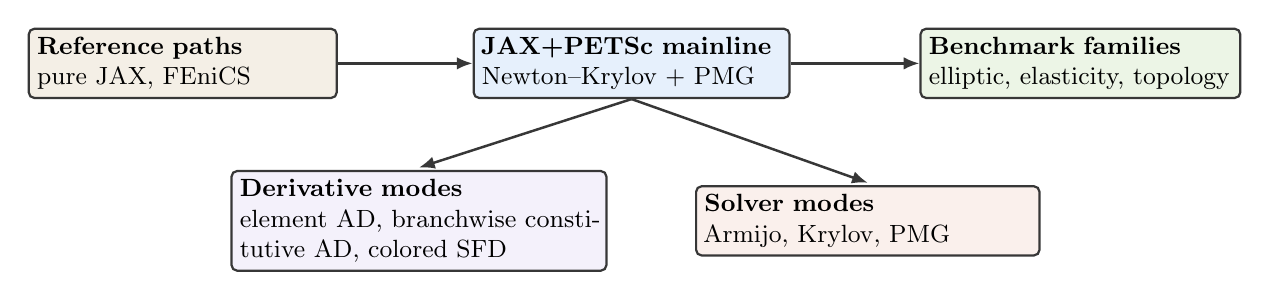
\begin{tikzpicture}[x=1cm,y=1cm]
  \node[paper box, fill=paperdiagbeige, text width=3.7cm] (ref) at (0,0)
    {\textbf{Reference paths}\\pure JAX, FEniCS};
  \node[paper box, fill=paperdiagblue, text width=3.8cm] (main) at (5.7,0)
    {\textbf{JAX+PETSc mainline}\\Newton--Krylov + PMG};
  \node[paper box, fill=paperdiaggreen, text width=3.85cm] (bench) at (11.4,0)
    {\textbf{Benchmark families}\\elliptic, elasticity, topology};
  \node[paper box, fill=paperdiagviolet, text width=4.55cm] (deriv) at (3.0,-2.0)
    {\textbf{Derivative modes}\\element AD, branchwise constitutive AD, colored SFD};
  \node[paper box, fill=paperdiagrose, text width=4.15cm] (solver) at (8.7,-2.0)
    {\textbf{Solver modes}\\Armijo, Krylov, PMG};

  \draw[paper arrow] (ref.east) -- (main.west);
  \draw[paper arrow] (main.east) -- (bench.west);
  \draw[paper arrow] (main.south) -- ($(deriv.north)+(0,0.03)$);
  \draw[paper arrow] (main.south) -- ($(solver.north)+(0,0.03)$);
\end{tikzpicture}%
}

\newcommand{\PaperDerivativePathDiagram}{%
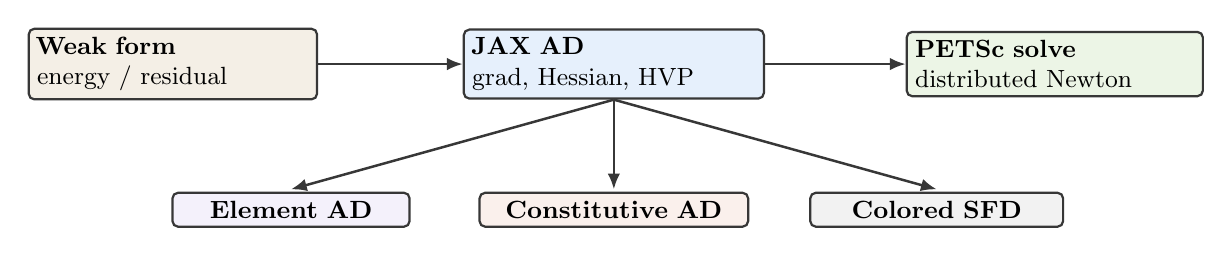
\begin{tikzpicture}[x=1cm,y=1cm]
  \node[paper box, fill=paperdiagbeige, text width=3.45cm] (weak) at (0,0)
    {\textbf{Weak form}\\energy / residual};
  \node[paper box, fill=paperdiagblue, text width=3.6cm] (jax) at (5.6,0)
    {\textbf{JAX AD}\\grad, Hessian, HVP};
  \node[paper box, fill=paperdiaggreen, text width=3.55cm] (petsc) at (11.2,0)
    {\textbf{PETSc solve}\\distributed Newton};

  \node[paper box, fill=paperdiagviolet, text width=2.8cm, align=center] (elem) at (1.5,-1.85)
    {\textbf{Element AD}};
  \node[paper box, fill=paperdiagrose, text width=3.2cm, align=center] (const) at (5.6,-1.85)
    {\textbf{Constitutive AD}};
  \node[paper box, fill=paperdiaggray, text width=3.0cm, align=center] (sfd) at (9.7,-1.85)
    {\textbf{Colored SFD}};

  \draw[paper arrow] (weak.east) -- (jax.west);
  \draw[paper arrow] (jax.east) -- (petsc.west);
  \draw[paper arrow] (jax.south) -- ($(elem.north)+(0,0.03)$);
  \draw[paper arrow] (jax.south) -- ($(const.north)+(0,0.03)$);
  \draw[paper arrow] (jax.south) -- ($(sfd.north)+(0,0.03)$);
\end{tikzpicture}%
}

\newcommand{\PaperAutodiffModesDiagram}{%
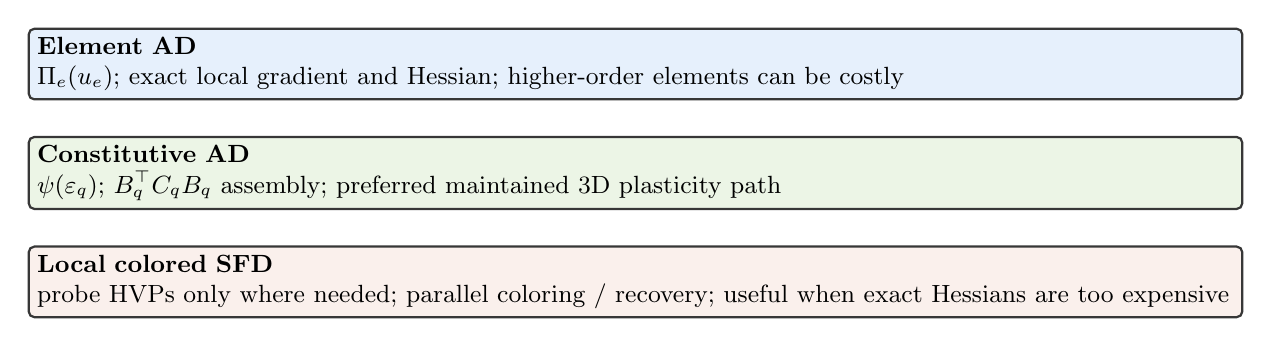
\begin{tikzpicture}[x=1cm,y=1cm]
  \node[paper box, fill=paperdiagblue, text width=15.2cm] (e) at (0,0)
    {\textbf{Element AD}\\$\Pi_e(u_e)$; exact local gradient and Hessian; higher-order elements can be costly};
  \node[paper box, fill=paperdiaggreen, text width=15.2cm, below=0.45cm of e] (c)
    {\textbf{Constitutive AD}\\$\psi(\varepsilon_q)$; $B_q^\top C_q B_q$ assembly; preferred maintained 3D plasticity path};
  \node[paper box, fill=paperdiagrose, text width=15.2cm, below=0.45cm of c] (s)
    {\textbf{Local colored SFD}\\probe HVPs only where needed; parallel coloring / recovery; useful when exact Hessians are too expensive};
\end{tikzpicture}%
}

\newcommand{\PaperGlobalizationDiagram}{%
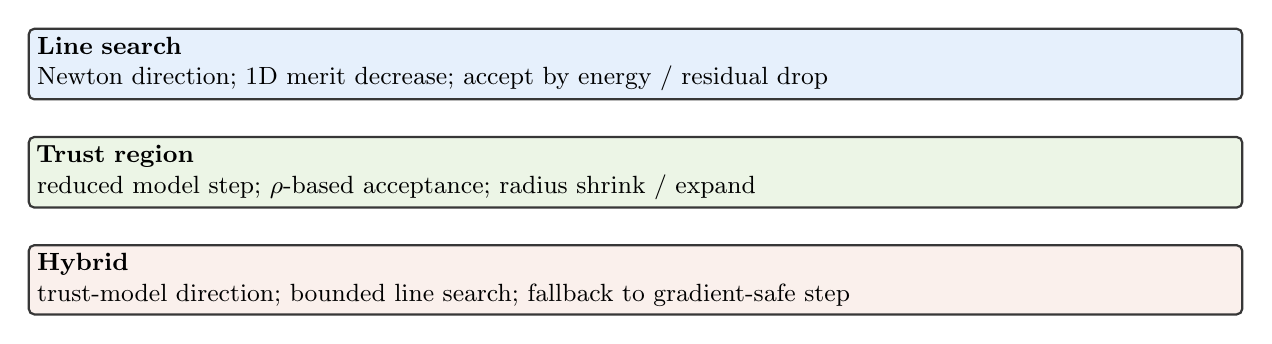
\begin{tikzpicture}[x=1cm,y=1cm]
  \node[paper box, fill=paperdiagblue, text width=15.2cm] (ls) at (0,0)
    {\textbf{Line search}\\Newton direction; 1D merit decrease; accept by energy / residual drop};
  \node[paper box, fill=paperdiaggreen, text width=15.2cm, below=0.45cm of ls] (tr)
    {\textbf{Trust region}\\reduced model step; $\rho$-based acceptance; radius shrink / expand};
  \node[paper box, fill=paperdiagrose, text width=15.2cm, below=0.45cm of tr] (hy)
    {\textbf{Hybrid}\\trust-model direction; bounded line search; fallback to gradient-safe step};
\end{tikzpicture}%
}

\newcommand{\PaperColoringDiagram}{%
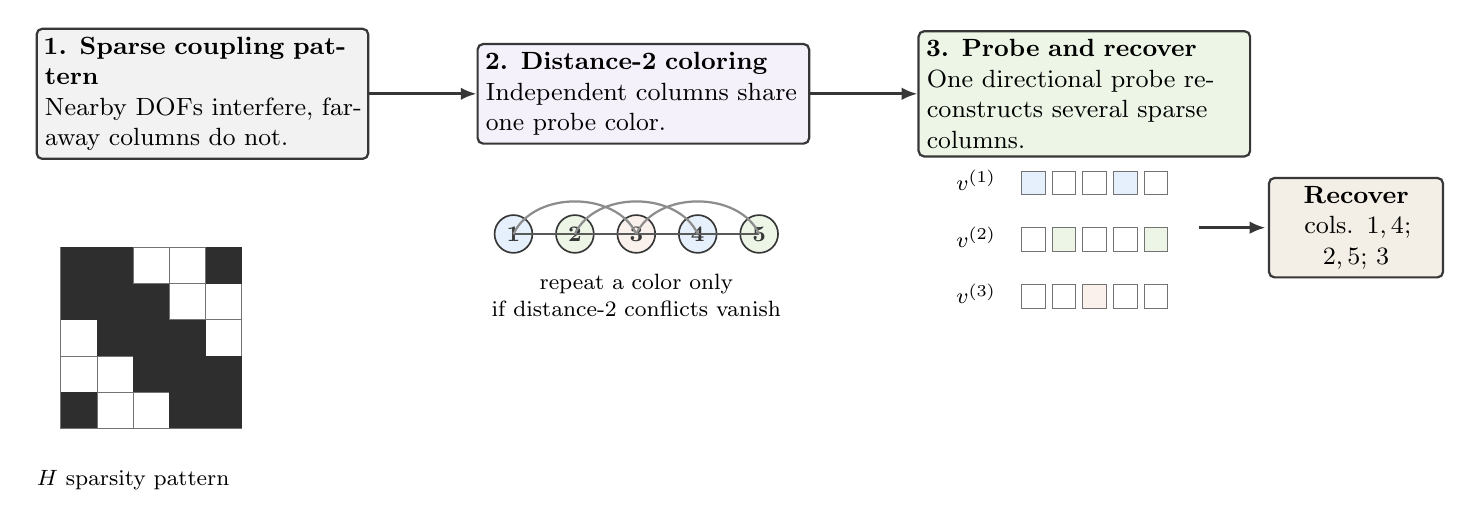
\begin{tikzpicture}[x=1cm,y=1cm]
  \tikzstyle{cell}=[draw=black!55, line width=0.30pt]
  \tikzstyle{stagearrow}=[paper arrow, line width=1.0pt]

  \node[paper box, fill=paperdiaggray, text width=4.0cm] (patternbox) at (0.0,0.0)
    {\textbf{1. Sparse coupling pattern}\\Nearby DOFs interfere, far-away columns do not.};
  \node[paper box, fill=paperdiagviolet, text width=4.0cm] (colorbox) at (5.6,0.0)
    {\textbf{2. Distance-2 coloring}\\Independent columns share one probe color.};
  \node[paper box, fill=paperdiaggreen, text width=4.0cm] (recoverbox) at (11.2,0.0)
    {\textbf{3. Probe and recover}\\One directional probe reconstructs several sparse columns.};

  \draw[stagearrow] (patternbox.east) -- (colorbox.west);
  \draw[stagearrow] (colorbox.east) -- (recoverbox.west);

  % Pattern panel
  \begin{scope}[shift={(-1.8,-1.95)}]
    \foreach \i in {0,...,4} {
      \foreach \j in {0,...,4} {
        \fill[white] (\i*0.46,-\j*0.46) rectangle ++(0.46,-0.46);
        \draw[cell] (\i*0.46,-\j*0.46) rectangle ++(0.46,-0.46);
      }
    }
    \foreach \i/\j in {
      0/0,1/0,0/1,1/1,
      1/2,2/1,2/2,2/3,3/2,3/3,
      3/4,4/3,4/4,
      0/4,4/0
    }{
      \fill[black!82] (\i*0.46,-\j*0.46) rectangle ++(0.46,-0.46);
    }
    \node[font=\footnotesize] at (0.92,-2.95) {$H$ sparsity pattern};
  \end{scope}

  % Coloring panel
  \begin{scope}[shift={(3.95,-1.78)}]
    \fill[paperdiagblue] (0.0,0) circle (0.24);
    \fill[paperdiaggreen] (0.78,0) circle (0.24);
    \fill[paperdiagrose] (1.56,0) circle (0.24);
    \fill[paperdiagblue] (2.34,0) circle (0.24);
    \fill[paperdiaggreen] (3.12,0) circle (0.24);
    \foreach \x/\lab in {0.0/1,0.78/2,1.56/3,2.34/4,3.12/5}{
      \draw[paperdiagdark,line width=0.6pt] (\x,0) circle (0.24);
      \node[font=\footnotesize\bfseries,text=paperdiagdark] at (\x,0) {\lab};
    }
    \draw[black!65,line width=0.8pt] (0.0,0) -- (0.78,0);
    \draw[black!65,line width=0.8pt] (0.78,0) -- (1.56,0);
    \draw[black!65,line width=0.8pt] (1.56,0) -- (2.34,0);
    \draw[black!65,line width=0.8pt] (2.34,0) -- (3.12,0);
    \draw[black!45,line width=0.8pt] (0.0,0) to[out=65,in=115] (1.56,0);
    \draw[black!45,line width=0.8pt] (0.78,0) to[out=65,in=115] (2.34,0);
    \draw[black!45,line width=0.8pt] (1.56,0) to[out=65,in=115] (3.12,0);
    \node[font=\footnotesize,align=center] at (1.56,-0.78) {repeat a color only\\if distance-2 conflicts vanish};
  \end{scope}

  % Recovery panel
  \begin{scope}[shift={(9.45,-2.08)}]
    \node[font=\footnotesize, anchor=west] at (0.00,0.98) {$v^{(1)}$};
    \node[font=\footnotesize, anchor=west] at (0.00,0.26) {$v^{(2)}$};
    \node[font=\footnotesize, anchor=west] at (0.00,-0.46) {$v^{(3)}$};
    \foreach \x in {0.95,1.34,1.73,2.12,2.51}{
      \fill[white] (\x,1.10) rectangle ++(0.30,-0.30);
      \draw[cell] (\x,1.10) rectangle ++(0.30,-0.30);
      \fill[white] (\x,0.38) rectangle ++(0.30,-0.30);
      \draw[cell] (\x,0.38) rectangle ++(0.30,-0.30);
      \fill[white] (\x,-0.34) rectangle ++(0.30,-0.30);
      \draw[cell] (\x,-0.34) rectangle ++(0.30,-0.30);
    }
    \fill[paperdiagblue] (0.95,1.10) rectangle ++(0.30,-0.30);
    \fill[paperdiagblue] (2.12,1.10) rectangle ++(0.30,-0.30);
    \fill[paperdiaggreen] (1.34,0.38) rectangle ++(0.30,-0.30);
    \fill[paperdiaggreen] (2.51,0.38) rectangle ++(0.30,-0.30);
    \fill[paperdiagrose] (1.73,-0.34) rectangle ++(0.30,-0.30);
    \draw[cell] (0.95,1.10) rectangle ++(0.30,-0.30);
    \draw[cell] (2.12,1.10) rectangle ++(0.30,-0.30);
    \draw[cell] (1.34,0.38) rectangle ++(0.30,-0.30);
    \draw[cell] (2.51,0.38) rectangle ++(0.30,-0.30);
    \draw[cell] (1.73,-0.34) rectangle ++(0.30,-0.30);
    \draw[stagearrow] (3.20,0.38) -- (4.05,0.38);
    \node[paper box, fill=paperdiagbeige, text width=2.0cm, align=center] at (5.2,0.38)
      {\textbf{Recover}\\cols. $1,4$;\\$2,5$; $3$};
  \end{scope}
\end{tikzpicture}%
}


\title{Nonlinear Finite-Element Solves and Optimization with JAX and PETSc:\\
\large Exact and Approximate Second-Order Routes\\
\large in a Maintained Sparse Solver Workflow}

\author{
\repo{} contributors\\
\small Manuscript draft; author and affiliation metadata to be supplied before submission
}

\date{\today}

\begin{document}

\maketitle
\begin{abstract}
We present \repo{} as a software-and-methods workflow for nonlinear finite-element
solves and optimization that spans \purejax{} references, \fenics{} references
where they exist, and a maintained distributed \jaxpetsc{} implementation.
Across the maintained benchmark suite we cover nonlinear scalar problems
($p$-Laplace and Ginzburg--Landau), large-deformation hyperelasticity,
two-dimensional and three-dimensional Mohr--Coulomb plasticity, and topology
optimization. The methodological focus is a solver-centric combination of JAX
for local differentiation with PETSc for sparse assembly, globalization,
Krylov solves, and preconditioning, together with three second-order routes:
element automatic differentiation, constitutive automatic differentiation, and
colored sparse finite-difference recovery.

The evidence is separated into validation and performance layers. For the
three-dimensional heterogeneous Plasticity3D benchmark, a same-case
source-faithfulness comparison against the source-style endpoint surrogate is
tight, with relative differences
\num{3.877e-5} in work, \num{3.517e-3} in displacement, and
\num{8.720e-3} in deviatoric-strain norm. A separate fixed-lambda
source-operator diagnostic uses the matched glued-bottom boundary contract and
passes the configured field-agreement thresholds, with
$u_{\max}(\lambda)$ relative $L^2$ difference \num{6.396e-6} and endpoint
displacement relative $L^2$ difference \num{8.299e-4}. This validates the
implemented endpoint surrogate within the tested fixed-load contract, but not
as a path-consistent replacement for an incremental elastoplastic history
solve. On the locked $P_4(L_1)$,
$\lambda_{\mathrm{sr}}=1.5$, 8-rank derivative ablation, constitutive AD has
the lowest median wall time among the three tested routes while reaching the
same terminal state as element AD and colored SFD. A serial hyperelastic
companion comparison against JAX-FEM on the same mesh and displacement schedule
passes a 5\% fairness gate with repository-energy and field differences below
$10^{-3}$; this evidence is hyperelastic-only.

The largest maintained distributed timing study remains the promoted
\plasticitythree{} study on $P_4(L_2)$ with \localpmg{}, which attains
$\num{18.05}\times$ end-to-end speedup on 32 MPI
ranks relative to one rank at the same promoted nonlinear target. The topology
optimization study complements this with a distributed design-and-mechanics
workflow that remains operational at $768\times 384$ resolution and 32 ranks.
Within that scoped evidence, the paper's contribution is a maintained
implementation pattern: derivative-rich local models, sparse nonlinear solver
policy, and distributed execution can be kept together in one reproducible
workflow across a heterogeneous family of FEM problems.
\end{abstract}


\section{Introduction}
Recent open-source finite-element and PDE-optimization frameworks cover
different parts of the workflow needed for nonlinear solves and design. High-level
finite-element systems such as \fenics{} and \code{DOLFINx} emphasize expressive
variational modeling together with compiled kernels and parallel assembly
\citep{logg2012fenicsbook,baratta2025dolfinx}. PDE-level adjoint frameworks
such as \code{dolfin-adjoint}, \code{pyadjoint}, and \code{cashocs} automate
adjoint-centered optimization workflows and PDE-level sensitivity automation
\citep{farrell2013dolfinadjoint,mitusch2019pyadjoint,blauth2023cashocsv2}.
JAX-native or JAX-connected workflows, including JAX-FEM, AutoPDEx,
JAX-CPFEM, the Firedrake--JAX bridge, and recent \code{FEniCSx} external-operator
work, push automatic differentiation deeper into constitutive modeling and
differentiable simulation
\citep{xue2023jaxfem,bode2025autopdex,hu2025jaxcpfem,yashchuk2023bringing,latyshev2025externaloperators}.
Recent topology-optimization implementations such as \code{FEniTop} show that
compact parallel design-mechanics workflows can also be built on modern
\code{FEniCSx} infrastructure \citep{jia2024fenitop}.

This paper targets a narrower design point than the broad differentiable-PDE
landscape above. The maintained production path in \repo{} is a solver-centric
\jaxpetsc{} stack for distributed nonlinear finite-element solves and optimization.
Local energies and constitutive laws are written in JAX, while sparse assembly,
globalization, Krylov solves, and preconditioning are handled by PETSc. The goal
is not to claim one universally preferred framework, but to document one specific
combination that is practically useful for our benchmark families: high-level
local differentiation coupled to distributed sparse Newton--Krylov execution on
hard nonlinear mechanics and design problems.

The central claim is therefore deliberately limited. We do not claim that every
benchmark requires exact Hessians, nor that mainstream frameworks cannot provide
them. We instead show that several derivative routes can be made operational
inside one maintained distributed workflow:
\begin{enumerate}
  \item exact element-level derivatives when the local state dimension is still
        affordable;
  \item constitutive-level automatic differentiation for high-order plasticity,
        where local tangents are much cheaper than full element Hessians;
  \item colored sparse finite-difference (SFD) recovery when exact second-order
        information is not the right cost-quality tradeoff.
\end{enumerate}

These routes are evaluated on six maintained benchmark families:
$p$-Laplace, scalar Ginzburg--Landau, hyperelasticity, Plasticity2D,
\plasticitythree{}, and topology optimization. The paper gives all six families
top-level space because the main contribution is methodological rather than a
single benchmark-specific solver. At the same time, \plasticitythree{} and
topology optimization receive the most detailed comparison because they are the
closest stress tests for the maintained \jaxpetsc{} path; \plasticitythree{} is
also the family in which source-faithfulness, surrogate interpretation, and
historical scaling have to be separated most carefully. The geomechanics context
for that family follows the finite-element strength-reduction and 3D
slope-stability literature \citep{tschuchnigg2015nonassociated,sysala2021optimization,sysala2025advancedcontinuation},
but the repository object studied here is explicitly the implemented endpoint
surrogate, not a claim of path-consistent incremental-history equivalence.

\subsection{State of the Art and Positioning}
\label{sec:intro-sota}

For the purposes of this paper, the most relevant comparison axes are the
modeling layer, the scope of differentiation, the form in which second-order
information enters the workflow, the parallel execution model, and the benchmark
families closest to our maintained suite. \Cref{tab:sota-comparison} summarizes
that comparison using conservative, source-backed descriptors.

\begin{table}[tbp]
  \centering
  \scriptsize
  \setlength{\tabcolsep}{3pt}
  \begin{tabular*}{\textwidth}{@{}>{\RaggedRight\arraybackslash}p{0.16\textwidth}@{\extracolsep{\fill}} >{\RaggedRight\arraybackslash}p{0.13\textwidth} >{\RaggedRight\arraybackslash}p{0.15\textwidth} >{\RaggedRight\arraybackslash}p{0.15\textwidth} >{\RaggedRight\arraybackslash}p{0.14\textwidth} >{\RaggedRight\arraybackslash}p{0.18\textwidth}@{}}
\toprule
Family & Modeling & Differentiation & Second-order route & Parallel & Closest overlap \\
\midrule
\shortstack[l]{FEniCS\\DOLFINx\\\citep{logg2012fenicsbook,baratta2025dolfinx}} & High-level variational forms & Problem-specific; AD is not the central claim & Manual or application-specific & Distributed FEM assembly and solve & Elliptic and finite-strain mechanics \\
\shortstack[l]{dolfin-adjoint\\pyadjoint\\cashocs\\\citep{farrell2013dolfinadjoint,mitusch2019pyadjoint,blauth2023cashocsv2}} & High-level PDE plus optimization loop & Adjoint-based first-order sensitivities & Not the advertised main path & MPI via the host FEM stack & PDE control, shape, and topology \\
\shortstack[l]{JAX-FEM\\AutoPDEx\\\citep{xue2023jaxfem,bode2025autopdex}} & JAX-native PDE / FE programs & Program-level forward and reverse AD & Higher-order JAX derivatives & JAX execution; PETSc optional in AutoPDEx & Nonlinear mechanics and inverse design \\
\shortstack[l]{Firedrake--JAX\\FEniCSx ext. ops\\\citep{yashchuk2023bringing,latyshev2025externaloperators}} & Host FEM stack plus AD bridge & Tangent, adjoint, or local constitutive AD & Local-operator derivatives, not full sparse Hessians & Host framework parallel back end & Parameterized PDEs and constitutive models \\
\shortstack[l]{JAX-CPFEM\\\citep{hu2025jaxcpfem}} & JAX-native crystal-plasticity FEM & Differentiable constitutive simulator & AD constitutive derivatives & GPU-oriented execution & Crystal plasticity \\
\shortstack[l]{FEniTop\\\citep{jia2024fenitop}} & FEniCSx topology code & Sensitivity-based design updates & Not a second-order solver paper & Parallel FEniCSx workflow & 2D and 3D topology optimization \\
This work & JAX local energies plus PETSc sparse solvers & Element AD, constitutive AD, and colored SFD & Local Hessians/tangents or sparse recovery & PETSc MPI vectors, matrices, SNES, and multigrid & $p$-Laplace, GL, hyperelasticity, plasticity, topology \\
\bottomrule
\end{tabular*}

  \caption{State-of-the-art positioning of the framework families most relevant
  to this paper. The columns record source-supported workflow properties rather
  than subjective scores.}
  \label{tab:sota-comparison}
\end{table}

Three comparisons matter most for the narrative that follows. First, relative to
high-level FEM and adjoint ecosystems
\citep{logg2012fenicsbook,baratta2025dolfinx,farrell2013dolfinadjoint,mitusch2019pyadjoint,blauth2023cashocsv2},
\repo{} moves the center of gravity from PDE-level adjoint-centered automation toward
distributed nonlinear solve policy and multiple second-order routes inside the
same sparse solver stack. Second, relative to JAX-native mechanics and
differentiable-simulation frameworks
\citep{xue2023jaxfem,bode2025autopdex,hu2025jaxcpfem}, the main distinction is
that the maintained implementation here centers PETSc-owned sparse MPI data
structures and preconditioned Newton solves, whereas the cited JAX-native
frameworks emphasize JAX-level modeling, local differentiation, GPU execution,
or implicit-differentiation workflows. Third, relative to recent bridge papers
that combine JAX-style differentiation with established FEM environments
\citep{yashchuk2023bringing,latyshev2025externaloperators}, the paper's emphasis
is on extending that bridge-style differentiation story into benchmarked PETSc
sparse assembly, Krylov solves, and nonlinear globalization for benchmark
families that include topology optimization and 3D Mohr--Coulomb-type
mechanics.

The resulting positioning statement is intentionally modest. \repo{} is not
presented as a general differentiable-PDE platform, nor as a replacement for the
high-level FEM and adjoint ecosystems cited above. It is presented as a
maintained JAX+PETSc workflow for distributed nonlinear energy minimization and
equilibrium solves in which derivative fidelity, sparse linear algebra, and
preconditioner policy are all part of the experimental design and comparison
criteria rather than merely implementation detail.

The paper is organized as follows. \Cref{sec:related} deepens the literature
context behind the summary above. \Cref{sec:methodology} describes the common
optimization and derivative machinery, including line search, trust regions, and
colored derivative recovery. \Cref{sec:implementation} explains how these ideas
are mapped onto \purejax{}, \fenics{}, and \jaxpetsc{}. \Cref{sec:benchmarks}
defines the benchmark suite, with each benchmark separated into literature model
and repository specialization. \Cref{sec:numerical-examples} then reports the
timing, scaling, and discretization-comparison evidence, followed by supporting
solver evidence and a discussion of limitations.


\section{Related Work}
\label{sec:related}

The literature most relevant to this manuscript falls into seven closely connected
groups: high-level finite-element automation, PDE-level adjoint optimization,
JAX-native differentiable FEM, JAX-to-FEM/PETSc bridge mechanisms,
Mohr--Coulomb slope-stability source-lineage context, topology optimization
workflows, and sparse nonlinear solver infrastructure. The purpose of this
section is not to assign a single ranking to those groups, but to state precisely
which part of each literature thread the present paper uses as context.

\paragraph{High-level finite-element automation.}
The original \fenics{} project established the high-level finite-element
programming model in which weak forms are expressed symbolically and compiled
into efficient kernels \citep{logg2012fenicsbook}. The more recent
\code{DOLFINx} preprint keeps that high-level mathematical abstraction while
moving to a data-oriented design with explicit support for modern parallelism,
custom kernels, and direct access to lower-level data structures
\citep{baratta2025dolfinx}. This literature defines the reference standard for
what an expressive open-source FEM environment should provide.

\paragraph{Adjoint-based PDE optimization.}
\code{dolfin-adjoint} showed that adjoints of high-level transient finite-element
programs can be derived automatically from the symbolic problem description
\citep{farrell2013dolfinadjoint}. The later \code{pyadjoint} software paper
documents the maintained FEniCS/Firedrake adjoint framework used to automate
such workflows in practice \citep{mitusch2019pyadjoint}. The present
\code{cashocs} software paper extends that PDE-constrained-optimization thread
to shape optimization, optimal control, topology optimization via level sets,
and MPI-enabled workflows \citep{blauth2023cashocsv2}. These works are the
right comparison point for adjoint-centered PDE-level automation and
optimization workflows, but they do not have the same focus as the present
paper on explicit second-order routes inside distributed sparse nonlinear solve
stacks.

\paragraph{JAX-native differentiable FEM.}
The broad AD background is surveyed by \citet{baydin2018autodiff}, while JAX
provides the program-transformation environment that makes higher-order
derivatives, vectorization, and just-in-time compilation readily usable in
scientific computing \citep{jax2018}. Within finite elements, JAX-FEM shows that
inverse design, nonlinear constitutive modeling, and GPU-oriented differentiable
workflows can be implemented inside a JAX-native 3D FE solver
\citep{xue2023jaxfem}. Xue's later finite-element differentiable-physics paper
is a direct second-order comparator because it derives implicit Hessian-vector
products and evaluates Newton-CG-style use of exact Hessian information on
finite-element inverse-problem benchmarks \citep{xue2026implicit}. AutoPDEx
broadens that JAX-native PDE picture with nonlinear minimizers, implicit
differentiation, and optional PETSc integration \citep{bode2025autopdex}.
JAX-CPFEM is especially relevant to the mechanics side of the present paper
because it couples differentiable FEM, nonlinear crystal plasticity, and GPU
execution in a recent open-access workflow \citep{hu2025jaxcpfem}. Together,
these papers define the closest modern literature context for the repository's
JAX-based local differentiation layer and second-order derivative comparisons.

\paragraph{Bridges between JAX-style AD and established FEM stacks.}
The Firedrake--JAX bridge of \citet{yashchuk2023bringing} is important because
it bypasses differentiation through low-level solver iterations by using
tangent-linear and adjoint equations derived from the high-level PDE
representation. The recent \code{FEniCSx} external-operator paper by
\citet{latyshev2025externaloperators} is even closer to the constitutive story
of this manuscript: it uses algorithmic automatic differentiation for general
constitutive models inside \code{FEniCSx}, including a Mohr--Coulomb example.
Those papers show that constitutive- or solve-level differentiation can be
combined with established FEM environments without differentiating every low-level
algebraic step. The present paper extends that bridge-style differentiation
story into a PETSc-centered sparse assembly and nonlinear-solve setting with
explicit comparison between element AD, constitutive AD, and colored SFD. The
JetSCI preprint is the closest recent hybrid in architecture: it uses JAX for
local finite-element discretization and PETSc for robust distributed sparse
solves in heterogeneous micromechanics \citep{cattaneo2026jetsci}. We therefore
treat it as evidence from a submitted preprint that the JAX-local/PETSc-global
split is an active design point, while keeping the present paper's claim
narrower: a maintained nonlinear energy-minimization suite with derivative-route
comparisons across the benchmark families below.

\paragraph{Mohr--Coulomb slope stability and source-lineage context.}
The plasticity benchmarks use Mohr--Coulomb-type slope-stability problems as
reviewer-visible stress tests, so their citations have to distinguish continuum
plasticity, strength-reduction practice, and repository-specific surrogates.
Davis' plasticity treatment and the finite-element strength-reduction studies of
\citet{tschuchnigg2015nonassociated} provide the Davis-style reduction context
used in the paper. For constitutive integration, the incremental reference frame
is return mapping with consistent tangents \citep{simo1985consistent,simo1998compinel},
with Mohr--Coulomb-specific nonsmooth return operators treated by
\citet{sysala2017returnmapping}. The recent Sysala slope-stability line also
documents variational and optimization viewpoints for shear strength reduction
\citep{sysala2021optimization,sysala2025convexoptimization} and a 3D
continuation/iterative-solver source family \citep{sysala2025advancedcontinuation}.
The present manuscript uses that literature to position the benchmark family,
while the numerical claims remain limited to the implemented surrogate and the
repository artifacts reported below.

\paragraph{Topology optimization workflows.}
The classical SIMP and educational topology-optimization references remain
important because they supply the baseline compliance, filtering, and
continuation ideas used throughout the field
\citep{sigmund2001topology,bendsoe2003topology,ferrari2020top99,bourdin2001filters}.
For the present paper, however, the more direct modern comparator is
\code{FEniTop}, which documents a simple 2D/3D \code{FEniCSx} topology-optimization
implementation with parallel support \citep{jia2024fenitop}. That paper is
relevant not because it duplicates our reduced design objective, which it does
not, but because it provides a recent source-backed baseline for how a compact
parallel topology-optimization code can be organized in the modern FEniCSx
ecosystem.

\paragraph{Sparse derivative recovery and scalable nonlinear infrastructure.}
When exact second-order information is too expensive, sparse derivative recovery
via graph coloring remains the classical alternative. Curtis, Powell, and Reid
gave the foundational sparse-Jacobian viewpoint \citep{curtis1974sparsejacobian},
while Coleman and Mor{\'e} extended the approach to sparse Jacobian and Hessian
estimation with graph-coloring structure
\citep{coleman1983sparsejacobian,coleman1984sparsehessian}. PETSc supplies the
distributed vectors, matrices, Krylov methods, nonlinear solvers, and multigrid
infrastructure needed to turn those derivative objects into scalable workflows
\citep{balay1997petsc,petsc2024web}. In this paper, PETSc is not treated as a
mere back-end library: ownership layout, Krylov policy, nonlinear globalization,
and preconditioner design are all part of the scientific comparison.

Against that background, the niche of \repo{} can be stated precisely. It sits
between high-level differentiable modeling and scalable sparse nonlinear solver
engineering. The contribution is not that it replaces the ecosystems above, but
that it documents one specific point in the contemporary design space:
maintained distributed nonlinear FEM workflows that combine JAX-based local
differentiation, multiple second-order routes, and PETSc-based sparse execution
on benchmark families ranging from scalar nonlinear diffusion to topology
optimization and 3D Mohr--Coulomb-type mechanics.


\section{Methodology}
\label{sec:methodology}

We use a common finite-element notation across all benchmark families. The
continuous domain is $\Omega \subset \mathbb{R}^d$, the conforming trial space
is $V_h \subset V$, the state vector is $u_h \in V_h$, and the element-restricted
state on element $e$ is $u_e$. When a family is posed as an energy or reduced
objective minimization, we write its discrete functional as
$\mathcal{J}_h(u_h)$; when a family is posed as a sequence of equilibrium
solves or by a scalar equilibrium surrogate, we write the associated scalar
functional as $\Pi_h(u_h)$.
Hyperelasticity is the only family in which $J=\det F$ denotes the deformation
Jacobian, so we avoid the bare symbol $J$ for generic objectives elsewhere in
the paper.
For finite-element labels, $P_k(L_\ell)$ denotes degree-$k$ Lagrange elements
on mesh level $L_\ell$; problem-specific sections define the mesh hierarchy
behind those levels when it matters for interpretation.

At the implementation level, the common sparse-assembly task is therefore one
of two closely related forms:
\begin{equation}
  \mathcal{J}_h(u_h)
  = \sum_{e=1}^{n_{\mathrm{el}}} \Phi_e(u_e) - f_{\mathrm{ext}}^T u_h,
  \label{eq:generic-objective}
\end{equation}
or
\begin{equation}
  \Pi_h(u_h)
  = \sum_{e=1}^{n_{\mathrm{el}}} \Phi_e(u_e) - f_{\mathrm{ext}}^T u_h,
  \label{eq:generic-potential}
\end{equation}
where $\Phi_e$ may represent a scalar diffusion energy, a phase-field
potential, a finite-strain stored-energy density, a repository scalarized
plasticity surrogate, or the reduced design objective used in topology
optimization. The benchmark
sections specialize \cref{eq:generic-objective,eq:generic-potential} to each
family and define any additional symbols locally.

\subsection{Finite-element and derivative structure}

The main design choice in \repo{} is that problem definitions should remain
energy-centered whenever possible. This gives three derivative routes:
\begin{enumerate}
  \item \textbf{element AD:} differentiate the full scalar element energy
        $\Pi_e(u_e)$ with respect to the element DOF vector;
  \item \textbf{constitutive AD:} differentiate a quadrature-point energy
        density $\psi(\varepsilon_q)$, then assemble
        $r_e = \sum_q w_q B_q^T \sigma_q$ and
        $K_e = \sum_q w_q B_q^T C_q B_q$;
  \item \textbf{colored SFD:} recover sparse Hessian information through
        directionally probed gradients/HVPs and graph coloring.
\end{enumerate}

Element AD is the most literal route and is often the cleanest mathematically.
Constitutive AD preserves the same scalar-energy source of truth but changes
the differentiation boundary from the full element vector to the local strain
state. This is especially effective for high-order plasticity, where the full
element Hessian is often much more expensive than the $6\times6$
constitutive tangent. Colored SFD is used when exact second-order information
is too costly or unnecessary.

\subsection{Newton--Krylov globalization}

The nonlinear solves in the repository are based on Newton or quasi-Newton
updates, but they are not all globalized in the same way. Scalar benchmarks
primarily use line-search Newton. Hyperelasticity uses a trust-region method
with optional post-step line search. Some maintained experiments use a hybrid
trust-region/line-search algorithm in which a reduced trust-region model
provides the direction, while a bounded line search chooses the accepted step.
The line-search and trust-region ingredients follow standard globalization ideas
\citep[Chs.~2--4]{nocedal2006numerical}; the particular hybrid coupling used in
some repository experiments is an implementation-specific combination of those
textbook ingredients.

\begin{algorithm}[H]
\caption{Hybrid trust-region / line-search Newton}
\begin{algorithmic}[1]
\State Given $x_0$, trust radius $\Delta_0$, tolerances, and callbacks for
energy, gradient, and Hessian solves/matvecs
\For{$k=0,1,\dots$}
  \State Assemble $g_k = \nabla J(x_k)$
  \If{convergence criteria are satisfied}
    \State terminate
  \EndIf
  \State Compute a Newton-like direction from $H(x_k)p = -g_k$
  \If{trust region is enabled}
    \State Build a small reduced model in the span of Newton and gradient directions
    \State Solve the reduced trust subproblem with radius $\Delta_k$
    \State Optionally compare against a pure gradient trust step
    \State Restrict the line-search interval so the accepted step stays in the trust ball
  \Else
    \State Use the Newton direction directly
  \EndIf
  \State Perform one-dimensional search on the chosen direction
  \State Compute actual and predicted reduction
  \If{trust region is enabled}
    \State accept/reject using $\rho = \mathrm{ared}/\mathrm{pred}$ and update $\Delta_k$
  \Else
    \State accept only if the merit function decreases
  \EndIf
\EndFor
\end{algorithmic}
\end{algorithm}

For the maintained 3D plasticity path promoted in this paper, the chosen policy
is simpler: Newton with Armijo backtracking and a PMG-preconditioned
\code{fgmres} linear solve \citep[Sec.~3.1]{nocedal2006numerical}. This is the
maintained baseline workflow used for the flagship benchmark reported later in
\Cref{sec:num-plasticity3d}.

\begin{algorithm}[H]
\caption{Armijo line search used in maintained Newton solves}
\begin{algorithmic}[1]
\State Given state $x$, direction $p$, initial step $\alpha_0$
\State Evaluate $J(x)$ and $g = \nabla J(x)$
\For{$m=0,1,\dots,m_{\max}$}
  \State $\alpha \gets \alpha_0 \beta^m$
  \State $x_{\mathrm{trial}} \gets x + \alpha p$
  \If{$J(x_{\mathrm{trial}}) \le J(x) + c_1 \alpha g^T p$}
    \State accept $\alpha$
    \State \Return
  \EndIf
\EndFor
\State fall back to the smallest admissible step or to gradient-safe logic
\end{algorithmic}
\end{algorithm}

\subsection{Colored sparse finite differences}

Sparse derivative recovery is built around the observation that if columns that
do not interfere in the sparsity pattern are perturbed together, one gradient
or HVP evaluation can recover multiple columns of the Jacobian or Hessian
\citep{curtis1974sparsejacobian,coleman1984sparsehessian}. In this repository,
the local SFD path uses distance-2 coloring on the Hessian sparsity graph,
which is especially effective when combined with overlap-domain assembly and
owned-plus-ghost PETSc layouts.

\begin{algorithm}[H]
\caption{Distributed colored Hessian recovery}
\begin{algorithmic}[1]
\State Build or import local sparsity information for the free-DOF graph
\State Compute a distance-2 coloring of the Hessian pattern
\For{each color group $c$}
  \State Build the combined probe vector $v_c$
  \State Evaluate one gradient difference or HVP for $v_c$
  \State Scatter recovered entries into owned sparse storage
\EndFor
\State Assemble the global PETSc matrix from owned COO/CSR entries
\end{algorithmic}
\end{algorithm}

\subsection{Constitutive autodiff for 3D plasticity}

The promoted \plasticitythree{} result in this paper uses constitutive AD.
Rather than applying second-order AD to the full $P4$ element vector, we write
one scalar Mohr--Coulomb energy density per quadrature point,
\begin{equation}
  \Phi_q(\varepsilon_q,\mathrm{material}_q),
\end{equation}
differentiate it with respect to the six engineering-strain components, and
assemble the element tangent from the resulting stress and constitutive tangent.
This keeps the scalar-energy contract intact while reducing the cost of
branchwise second-order information on high-order tetrahedra.

\begin{algorithm}[H]
\caption{Constitutive AD assembly for high-order plasticity}
\begin{algorithmic}[1]
\For{each local element $e$}
  \For{each quadrature point $q$}
    \State Evaluate strain $\varepsilon_q = B_q u_e$
    \State Evaluate scalar energy density $\Phi_q(\varepsilon_q)$
    \State Obtain stress $\sigma_q = \partial \Phi_q / \partial \varepsilon_q$
    \State Obtain constitutive tangent $C_q = \partial^2 \Phi_q / \partial \varepsilon_q^2$
  \EndFor
  \State Assemble $r_e = \sum_q w_q B_q^T \sigma_q$
  \State Assemble $K_e = \sum_q w_q B_q^T C_q B_q$
\EndFor
\end{algorithmic}
\end{algorithm}

The key methodological point is that automatic differentiation is applied
directly to the implemented scalar branch potential. The code does not switch
to a hand-derived constitutive tangent. Away from branch switching sets this
yields branchwise exact derivatives of the implemented surrogate; at switching
sets the model remains nonsmooth, so the resulting tangents should be read as
branchwise surrogate derivatives rather than globally smooth continuum
derivatives.


\section{Implementation}
\label{sec:implementation}

The repository intentionally keeps three implementation strata.

\paragraph{Pure JAX reference paths.}
These are the most compact differentiable implementations in the codebase.
They are useful for formulation checks, serial references, and debugging AD
logic. They are not intended to be the primary production route for the largest
distributed benchmarks. Their main scientific role in this paper is to show
that the energy formulations used in the maintained stack can also be expressed
in a compact differentiable form without sparse distributed infrastructure.

\paragraph{FEniCS reference paths.}
The \fenics{} implementations remain valuable on families where they exist,
especially $p$-Laplace, Ginzburg--Landau, and hyperelasticity. They provide a
trusted high-level FEM reference and help distinguish modeling issues from
solver-stack issues. In this repository they are used mainly as
comparison baselines rather than as the mainline production path.

\paragraph{Maintained \jaxpetsc{} path.}
This is the central implementation of the paper. It combines JAX-based local
physics with PETSc distributed vectors, matrices, Krylov solvers, and
preconditioners. Problem-specific kernels stay in JAX; sparse distributed
assembly, nonlinear globalization, and linear algebra stay in PETSc.

\subsection{Autodiff modes}

The maintained stack supports several second-order modes. The precise available
choices depend on the benchmark family, but the common logic is:
\begin{itemize}
  \item \textbf{element AD}: exact local Hessians from differentiating the full
        element energy;
  \item \textbf{constitutive AD}: exact local constitutive tangents assembled
        from quadrature-point energy densities;
  \item \textbf{local SFD / colored SFD}: sparse approximate Hessian recovery
        when exact second-order information is not the appropriate cost tradeoff.
\end{itemize}

This split is scientifically important. It lets us compare exact second-order
information against carefully structured sparse approximations without changing
the rest of the nonlinear solver stack. In other words, the paper is not only a
comparison of frameworks, but also a comparison of derivative strategies inside
one common solver infrastructure.

\begin{figure}[H]
  \centering
  \PaperFrameworkOverviewDiagram
  \caption{Software structure of the manuscript. The maintained \jaxpetsc{}
  implementation is the main production path; \purejax{} and \fenics{} remain
  reference paths where they already exist in the repository.}
  \label{fig:framework-overview}
\end{figure}

\begin{figure}[H]
  \centering
  \PaperDerivativePathDiagram
  \caption{Derivative pathways from scalar energies and quadrature-point
  potentials to distributed PETSc nonlinear solves.}
  \label{fig:derivative-pathways}
\end{figure}

\begin{figure}[H]
  \centering
  \PaperAutodiffModesDiagram
  \caption{Second-order derivative modes exposed in the maintained stack. The
  important engineering choice is that the source of truth remains an energy or
  energy-density expression even when the tangent path changes from element AD
  to constitutive AD or colored SFD.}
  \label{fig:derivative-stack}
\end{figure}

\subsection{Linear solvers and preconditioners}

The maintained families use different Krylov and preconditioner combinations
because the linear systems are qualitatively different:
\begin{itemize}
  \item \textbf{$p$-Laplace:} mostly \code{cg + hypre}, with exact element
        Hessians or local-SFD Hessians in the \jaxpetsc{} path.
  \item \textbf{Ginzburg--Landau:} \code{gmres + hypre}, reflecting the more
        indefinite linearization.
  \item \textbf{Hyperelasticity:} trust-region outer iterations with
        \code{gamg}-preconditioned Krylov solves.
  \item \textbf{Plasticity (2D):} deep-tail multigrid hierarchies whose
        bottlenecks are dominated by the top smoother and repeated Krylov
        work.
  \item \textbf{Plasticity3D:} local PMG on same-mesh
        \code{P4 -> P2 -> P1}, coarse \code{cg + hypre}, and an elastic initial
        guess on the same hierarchy.
  \item \textbf{Topology:} \code{fgmres + gamg} for the mechanics step, coupled
        to a separate distributed design update.
\end{itemize}

The comparison material later in the manuscript also includes a source-repo PMG-shell
variant and deflated GMRES. Those are not the primary maintained defaults, but
they are informative because they reveal how much of the final performance
difference comes from derivative paths, preconditioners, or outer solver logic.

\subsection{Distributed assembly and coloring}

The \jaxpetsc{} implementation uses PETSc-owned ranges, local-plus-ghost
layouts, and owned-row sparse assembly. This matters for both exact and
approximate second-order information. Exact element or constitutive assembly can
write directly into local sparse buffers. Colored SFD requires an additional
graph-coloring step, but once the coloring is known the probe evaluations can
still be carried out in a rank-local manner with only scalar reductions or
owned sparse insertion in the hot loop.

\begin{figure}[H]
  \centering
  \PaperGlobalizationDiagram
  \caption{Globalization choices used across the repository, from pure line
  search to trust-region and hybrid strategies.}
  \label{fig:globalization}
\end{figure}

\begin{figure}[H]
  \centering
  \PaperColoringDiagram
  \caption{Schematic view of the colored sparse-recovery logic used by the
  local SFD Hessian path: a sparsity pattern, a distance-2 coloring, and the
  corresponding grouped probes used for recovery.}
  \label{fig:globalization-coloring}
\end{figure}

\begin{table}[H]
  \centering
  \begin{tabular}{@{}l c c c >{\RaggedRight\arraybackslash}p{0.38\textwidth}@{}}
\toprule
Family & FEniCS & pure JAX & JAX+PETSc & Higher-order / advanced AD \\
\midrule
$p$-Laplace & yes & yes & yes & element AD and local colored SFD \\
Ginzburg--Landau & yes & no & yes & element AD and local colored SFD \\
Hyperelasticity & yes & yes & yes & trust-region element AD \\
Plasticity2D & no & no & yes & repository scalarized potential and same-mesh PMG \\
Plasticity3D & no & no & yes & constitutive AD, element AD, and same-mesh PMG \\
Topology optimization & no & yes & yes & distributed design updates and PETSc mechanics \\
\bottomrule
\end{tabular}

  \caption{Implementation capability matrix across the maintained benchmark
  families. ``Higher-order / advanced AD'' summarizes the derivative choices
  that are scientifically interesting in each family.}
  \label{tab:capability-matrix}
\end{table}

\Cref{tab:capability-matrix} summarizes the implemented surface. The most
important structural point is that the maintained production story is always
the \jaxpetsc{} column, even when a family also has \fenics{} or \purejax{}
references.


\section{Benchmark Problems}
\label{sec:benchmarks}

The benchmark suite is intentionally heterogeneous. The central claim of the
paper is not that one solver policy dominates every nonlinear PDE family, but
that one maintained differentiable sparse-solver stack can cover scalar
elliptic problems, phase-field-type energies, finite-strain mechanics,
elastoplastic slope stability, and reduced topology optimization without
switching conceptual frameworks.

\begin{table}[H]
  \centering
  \begin{tabular}{@{}l c >{\RaggedRight\arraybackslash}p{0.14\textwidth} >{\RaggedRight\arraybackslash}p{0.23\textwidth} >{\RaggedRight\arraybackslash}p{0.26\textwidth}@{}}
\toprule
Family & Grid / mesh & Stop rule & Compared paths & Main difficulty \\
\midrule
$p$-Laplace & $L_{9}$ & Newton + line search & FEniCS, pure JAX, JAX+PETSc & nonlinear elliptic solve with exact sparse Hessians \\
Ginzburg--Landau & $L_{9}$ & Newton + line search & FEniCS, JAX+PETSc & indefinite local curvature from the double well \\
Hyperelasticity & $L_{4}$, 24 steps & trust-region path & FEniCS, pure JAX, JAX+PETSc & nonconvex large-deformation mechanics \\
Plasticity2D & $P_{4}(L_{5})$--$P_{4}(L_{7})$ & endpoint or fixed work & JAX+PETSc only & same-mesh PMG and nonlinear tail behavior \\
Plasticity3D & $P_{1}$/$P_{2}$/$P_{4}$ & $\|g\| < \num{0.01}$ & constitutive-AD and source PMG variants & heterogeneous 3D Mohr--Coulomb with constitutive AD \\
Topology & $768\times384$ & stall-stop continuation & pure JAX, JAX+PETSc & distributed design-mechanics coupling \\
\bottomrule
\end{tabular}

  \caption{Benchmark families, stopping rules, and principal comparison paths.
  The later numerical section revisits the same families from the timing and
  scaling viewpoint.}
  \label{tab:benchmark-spec}
\end{table}

\begin{table}[H]
  \centering
  \begin{tabularx}{\textwidth}{@{}>{\hsize=1.080\hsize\linewidth=\hsize\RaggedRight\arraybackslash}X@{\hspace{0.8em}}>{\hsize=0.580\hsize\linewidth=\hsize\Centering\arraybackslash}X@{\hspace{0.7em}}>{\hsize=0.620\hsize\linewidth=\hsize\Centering\arraybackslash}X@{\hspace{1.0em}}>{\hsize=1.720\hsize\linewidth=\hsize\RaggedRight\arraybackslash}X@{}}
\toprule
Family & FEniCS & pure JAX & Notes \\
\midrule
$p$-Laplace & yes & yes & All three stacks exist on maintained showcase cases. \\
Ginzburg--Landau & yes & no & FEniCS and JAX+PETSc form the maintained comparison. \\
Hyperelasticity & yes & yes & pure JAX is a serial formulation reference only. \\
Plasticity2D & no & no & The maintained story is JAX+PETSc only. \\
Plasticity3D & no & no & Source assembly exists as supporting comparison, not as a maintained reference path. \\
Topology & no & yes & Parallel fine-grid path is JAX+PETSc; pure JAX remains the serial design reference. \\
\bottomrule
\end{tabularx}

  \caption{Availability of \fenics{} and \purejax{} references. Reference
  paths are used where the repository already provides documented implementations;
  absent cells are left absent rather than filled with speculative baselines.}
  \label{tab:reference-availability}
\end{table}

\subsection{\texorpdfstring{$p$-Laplace}{p-Laplace}}
\label{sec:bench-plaplace}

The literature model is the standard stationary $p$-Laplace Dirichlet problem
and its associated energy formulation \citep[Ch.~2]{lindqvist2019plaplace}. The
unknown is a scalar field $u:\Omega \to \mathbb{R}$ and the continuous energy is
\begin{equation}
  \mathcal{E}(u)
  = \int_{\Omega} \frac{1}{p} \lvert \nabla u \rvert^p \, dx
    - \int_{\Omega} f u \, dx,
  \label{eq:plaplace-energy}
\end{equation}
whose Euler--Lagrange equation is
\begin{equation}
  -\nabla \cdot \left(\lvert \nabla u \rvert^{p-2} \nabla u \right) = f
  \quad \text{in }\Omega,
  \qquad
  u = 0 \quad \text{on }\partial\Omega.
  \label{eq:plaplace-strong}
\end{equation}
The weak problem is: find $u \in W_0^{1,p}(\Omega)$ such that
\begin{equation}
  \int_{\Omega}
    \lvert \nabla u \rvert^{p-2} \nabla u \cdot \nabla v \, dx
  =
  \int_{\Omega} f v \, dx
  \qquad \forall v \in W_0^{1,p}(\Omega),
  \label{eq:plaplace-weak}
\end{equation}
The repository specialization used in this paper takes
$\Omega = (0,1)^2$, exponent $p=3$, forcing $f=-10$, and a conforming $P_1$
triangular hierarchy. The discrete problem is
\begin{equation}
  u_h \in V_h \subset W_0^{1,p}(\Omega):
  \qquad
  u_h = \arg\min_{v_h \in V_h} \mathcal{E}_h(v_h),
  \label{eq:plaplace-discrete}
\end{equation}
where $V_h$ is the chosen conforming finite-element subspace. This is the
cleanest benchmark in the paper for checking exact gradients, exact Hessians,
and sparse-recovery alternatives against each other without constitutive or
geometric complications.

\begin{figure}[H]
  \centering
  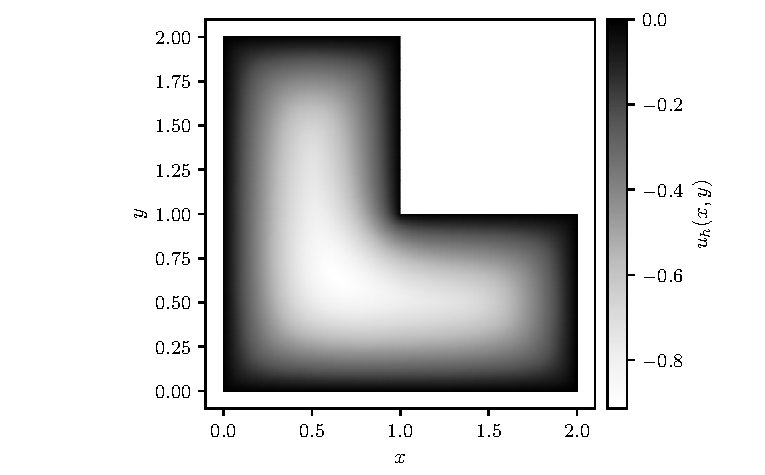
\includegraphics[width=\PaperFigureNarrow]{plaplace_state.pdf}
  \caption{Representative $p$-Laplace state on the maintained hierarchy.}
  \label{fig:plaplace-state}
\end{figure}

\begin{figure}[H]
  \centering
  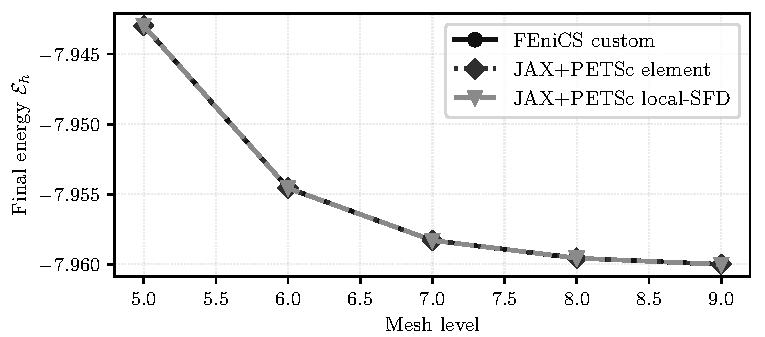
\includegraphics[width=\PaperFigureNarrow]{plaplace_energy_levels.pdf}
  \caption{Final discrete energies from \cref{eq:plaplace-discrete} across the
  maintained mesh hierarchy. The element-AD and local-SFD \jaxpetsc{} paths are
  essentially energy-consistent with the \fenics{} reference.}
  \label{fig:plaplace-energy-levels}
\end{figure}

\begin{table}[H]
  \centering
  \begin{tabular*}{\textwidth}{@{}l@{\extracolsep{\fill}} c c c c@{}}
\toprule
Path & Energy & Newton iters & Krylov iters & Wall time [s] \\
\midrule
FEniCS custom Newton & \num{-7.942968719} & 5 & 15 & \num{0.0782} \\
JAX+PETSc element AD & \num{-7.942968719} & 6 & 17 & \num{0.0798} \\
JAX+PETSc colored SFD & \num{-7.942968711} & 6 & 6 & \num{0.194} \\
\bottomrule
\end{tabular*}

  \caption{Representative final discrete energies from
  \cref{eq:plaplace-discrete} on the showcase case.}
  \label{tab:plaplace-benchmark}
\end{table}

The benchmark-local picture is therefore one of formulation agreement:
\cref{fig:plaplace-energy-levels,tab:plaplace-benchmark} show that the
maintained routes converge to the same discrete energy from
\cref{eq:plaplace-discrete}. Scaling and timing for this family are reported in
\Cref{sec:num-plaplace}.

\subsection{Ginzburg--Landau}
\label{sec:bench-gl}

We cite \citet{ginzburg1950theory} for the historical origin of
Ginzburg--Landau free-energy modeling only. The maintained benchmark used here is a
repository specialization: a scalar real-valued double-well problem on
$\Omega = [-1,1]^2$ with homogeneous Dirichlet boundary conditions and energy
\begin{equation}
  \mathcal{E}(u)
  =
  \int_{\Omega}
    \frac{\varepsilon}{2} \lvert \nabla u \rvert^2
    + \frac{1}{4}(u^2 - 1)^2 \, dx,
  \qquad
  \varepsilon = 10^{-2}.
  \label{eq:gl-energy}
\end{equation}
Its strong form is
\begin{equation}
  -\varepsilon \Delta u + u(u^2 - 1) = 0
  \quad \text{in }\Omega,
  \qquad
  u = 0 \quad \text{on }\partial\Omega,
  \label{eq:gl-strong}
\end{equation}
and the weak problem is: find $u \in H_0^1(\Omega)$ such that
\begin{equation}
  \int_{\Omega}
    \varepsilon \nabla u \cdot \nabla v
    + (u^2 - 1) u v \, dx
  = 0
  \qquad \forall v \in H_0^1(\Omega).
  \label{eq:gl-weak}
\end{equation}
The maintained discrete problem is a conforming $P_1$ stationary problem on the
same triangular hierarchy:
\begin{equation}
  u_h \in V_h:
  \qquad
  D\mathcal{E}_h(u_h)[v_h] = 0
  \qquad \forall v_h \in V_h.
  \label{eq:gl-discrete}
\end{equation}
Relative to $p$-Laplace, the additional difficulty here is not geometry but
indefinite local curvature from the double-well potential in
\cref{eq:gl-energy}.

\begin{figure}[H]
  \centering
  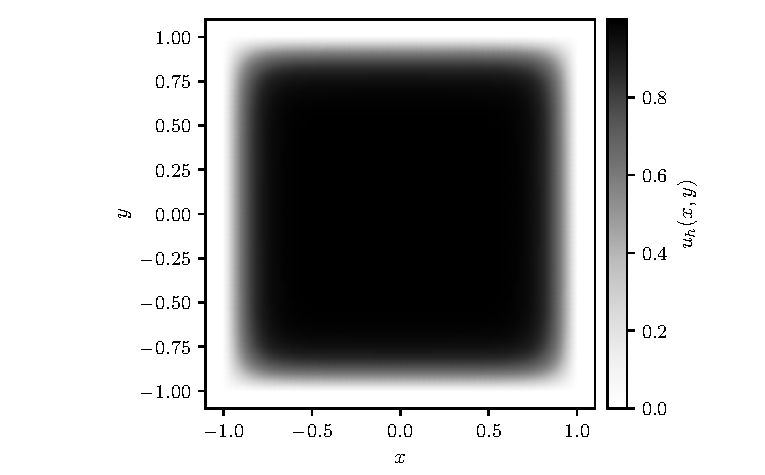
\includegraphics[width=\PaperFigureNarrow]{ginzburg_landau_state.pdf}
  \caption{Representative Ginzburg--Landau state on the maintained hierarchy.}
  \label{fig:gl-state}
\end{figure}

\begin{figure}[H]
  \centering
  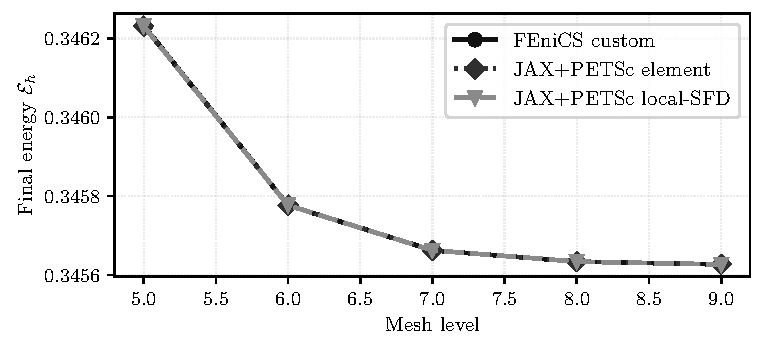
\includegraphics[width=\PaperFigureNarrow]{ginzburg_landau_energy_levels.pdf}
  \caption{Final discrete energies associated with the stationary problem
  \cref{eq:gl-discrete} across mesh
  levels. The maintained element-AD and local-SFD routes remain nearly
  coincident with the \fenics{} reference.}
  \label{fig:gl-energy-levels}
\end{figure}

\begin{table}[H]
  \centering
  \begin{tabular*}{\textwidth}{@{}l@{\extracolsep{\fill}} c c c c@{}}
\toprule
Path & Energy & Newton iters & Krylov iters & Wall time [s] \\
\midrule
FEniCS custom Newton & \num{0.3462323651} & 8 & 33 & \num{0.113} \\
JAX+PETSc element AD & \num{0.3462314438} & 8 & 33 & \num{0.0949} \\
JAX+PETSc colored SFD & \num{0.3462314438} & 8 & 33 & \num{0.247} \\
\bottomrule
\end{tabular*}

  \caption{Representative final discrete energies associated with
  \cref{eq:gl-discrete} on the showcase case.}
  \label{tab:gl-benchmark}
\end{table}

The local picture is again one of formulation consistency, now for a more
solver-sensitive nonconvex energy. Strong scaling and solver-time comparisons
for this family are reported in \Cref{sec:num-gl}.

\subsection{Hyperelasticity}
\label{sec:bench-he}

The literature model is a standard finite-strain hyperelastic equilibrium
problem written in terms of deformation map $y(X) = X + u(X)$, deformation
gradient $F = \nabla y$, Jacobian $J = \det F$, and first Piola stress
$P = \partial W / \partial F$ \citep[Chs.~4--6]{bonet2008nonlinear}. The
repository specialization used in this paper is a cantilever benchmark with the
compressible Neo-Hookean-type density
\begin{equation}
  \Pi(y;\eta)
  =
  \int_{\Omega}
    C_1 \left( \operatorname{tr}(F^T F) - 3 - 2 \ln J \right)
    + D_1 (J - 1)^2 \, dx,
  \label{eq:hyperelasticity-energy}
\end{equation}
on $\Omega = [0,0.4] \times [-0.005,0.005]^2$ with
$C_1 = \num{3.8461538461538464e7}$ and
$D_1 = \num{8.333333333333333e7}$. The left face is clamped, while the right
face carries the prescribed rotating Dirichlet load path used throughout the
repository, parametrized by load step $\eta$. The strong form is
\begin{equation}
  -\nabla \cdot P(F) = 0 \quad \text{in }\Omega,
  \qquad
  y = \bar y(\eta) \quad \text{on }\Gamma_D,
  \qquad
  P(F) n = 0 \quad \text{on }\Gamma_N,
  \label{eq:hyperelasticity-strong}
\end{equation}
where $P = \partial W / \partial F$ is the first Piola stress. The weak form is:
find $u \in V_{\bar y(\eta)}$ such that
\begin{equation}
  \int_{\Omega} P(F(u)) : \nabla v \, dx = 0
  \qquad \forall v \in V_0.
  \label{eq:hyperelasticity-weak}
\end{equation}
The discrete problem solved in the paper is the sequence of stationary points
\begin{equation}
  u_h^{(k)} \in V_h:
  \qquad
  D\Pi_h(u_h^{(k)};\eta_k)[v_h] = 0
  \qquad \forall v_h \in V_{h,0},
  \qquad
  k = 1,\dots,24,
  \label{eq:hyperelasticity-discrete}
\end{equation}
with first-order tetrahedral vector elements and the benchmark-specific boundary
data described above. This is the first family in which globalization is more
scientifically important than derivative parity alone.

\begin{figure}[H]
  \centering
  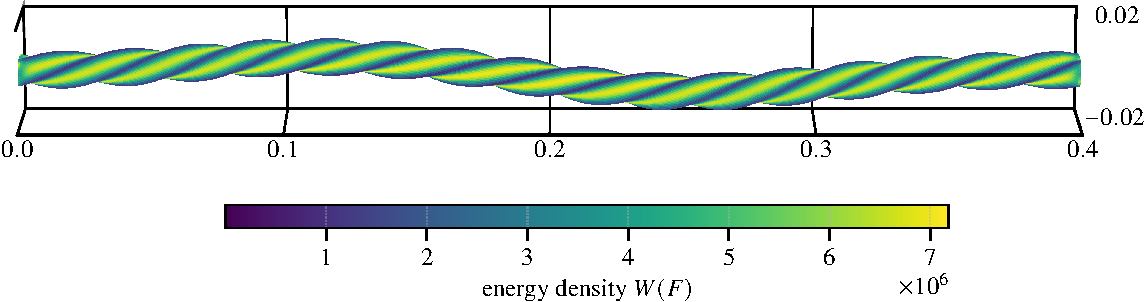
\includegraphics[width=\PaperFigureMedium]{hyperelasticity_state.pdf}
  \caption{Representative finite-strain hyperelastic state, colored by the
  energy density in \cref{eq:hyperelasticity-energy}.}
  \label{fig:hyperelasticity-state}
\end{figure}

\begin{figure}[H]
  \centering
  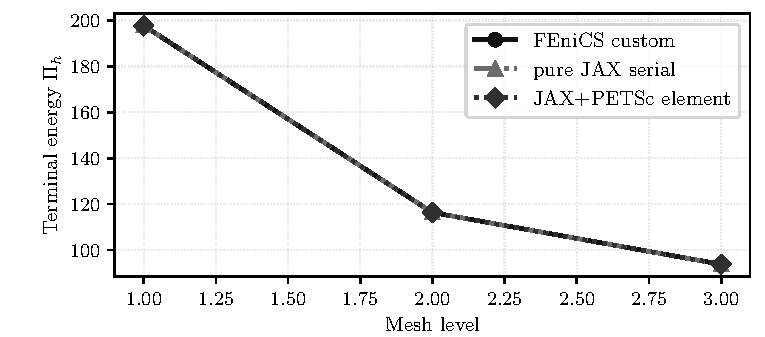
\includegraphics[width=\PaperFigureNarrow]{hyperelasticity_energy_levels.pdf}
  \caption{Final discrete energies along the stationary sequence
  \cref{eq:hyperelasticity-discrete} across the maintained mesh hierarchy. The
  publication story is less about
  exact equality than about tracking the same 24-step trajectory consistently.}
  \label{fig:hyperelasticity-energy-levels}
\end{figure}

\begin{table}[H]
  \centering
  \begin{tabular*}{\textwidth}{@{}l@{\extracolsep{\fill}} c c c c@{}}
\toprule
Path & Energy & Steps & Krylov iters & Wall time [s] \\
\midrule
FEniCS custom Newton & \num{197.775074} & 24 & 8722 & \num{6.51} \\
JAX+PETSc element AD & \num{197.754582} & 24 & 10595 & \num{9.36} \\
serial JAX & \num{197.749509} & 24 & 2284 & \num{41.5} \\
\bottomrule
\end{tabular*}

  \caption{Representative 24-step terminal energies along
  \cref{eq:hyperelasticity-discrete}.}
  \label{tab:hyperelasticity-benchmark}
\end{table}

The benchmark-local takeaway is therefore a globalization result:
\cref{fig:hyperelasticity-state,fig:hyperelasticity-energy-levels} show the
terminal deformed state and terminal energies, while the scaling evidence is
deferred to \Cref{sec:num-hyperelasticity}. That later section also adds one
matched serial companion baseline against JAX-FEM on the same mesh, material
law, and displacement schedule; it is included as a fairness-first
implementation comparison rather than as a broad framework ranking exercise.

\subsection{Plasticity2D}
\label{sec:bench-plasticity2d}

The literature model is a quasi-static plane-strain Mohr--Coulomb slope
stability problem posed as equilibrium together with a constitutive update and
history variables
\citep{davis1968plasticity,simo1985consistent,simo1998compinel,tschuchnigg2015nonassociated,sysala2017returnmapping,sysala2021optimization}.
The unknown is the displacement field
$u = (u_x,u_y):\Omega \to \mathbb{R}^2$ on the maintained homogeneous slope
geometry. At increment $n+1$, the continuum equilibrium equations are
\begin{equation}
  -\nabla \cdot \sigma^{n+1} = b^{n+1}
  \quad \text{in }\Omega,
  \qquad
  u^{n+1} = \bar u^{n+1} \quad \text{on }\Gamma_D,
  \qquad
  \sigma^{n+1}n = t^{n+1} \quad \text{on }\Gamma_N,
  \label{eq:plasticity2d-strong}
\end{equation}
where $\sigma^{n+1}$ and the internal variables are obtained from the
elastoplastic update driven by $\varepsilon(u^{n+1})$ and the previous state.
The corresponding weak form is
\begin{equation}
  \int_{\Omega} \sigma^{n+1} : \varepsilon(v) \, dx
  =
  \int_{\Omega} b^{n+1} \cdot v \, dx
  + \int_{\Gamma_N} t^{n+1} \cdot v \, ds
  \qquad \forall v \in V_0.
  \label{eq:plasticity2d-weak}
\end{equation}
The maintained runs reported here are endpoint solves, not path-consistent
incremental histories. Accordingly, the repository benchmark uses the following
scalarized discrete surrogate functional for differentiation and comparison:
\begin{equation}
  \Pi_h^{2\mathrm{D}}(u_h;\lambda_{\mathrm{sr}})
  =
  \sum_{e=1}^{n_{\mathrm{el}}}
  \sum_{q=1}^{n_q}
    w_{eq}\,
    \Phi_{\mathrm{MC},2\mathrm{D}}
    \!\left(
      B_{eq}u_e,\varepsilon^{p,\mathrm{old}}_{eq},
      E,\nu,c_{\lambda,eq},\phi_{\lambda,eq},\psi_{\lambda,eq}
    \right)
  - f_{\mathrm{ext}}^T u_h,
  \label{eq:plasticity2d-discrete}
\end{equation}
where $\lambda_{\mathrm{sr}}$ denotes the strength-reduction factor, distinct
from the Lam{\'e} parameter used later in three dimensions.

The maintained code keeps a Davis-B-style reduction path to map the raw
cohesion and angles to reduced values under strength reduction; with
$c_0,\phi,\psi$ denoting the unreduced cohesion, friction angle, and dilation
angle, respectively, the benchmark uses
\begin{align}
  c_1 &= c_0 / \lambda_{\mathrm{sr}},
  &
  \phi_1 &= \arctan \!\left(\tan \phi / \lambda_{\mathrm{sr}}\right),
  &
  \psi_1 &= \arctan \!\left(\tan \psi / \lambda_{\mathrm{sr}}\right),
  \nonumber\\
  \beta &= \frac{\cos \phi_1 \cos \psi_1}{1 - \sin \phi_1 \sin \psi_1},
  &
  c_{\lambda} &= \beta c_1,
  &
  \phi_{\lambda} &= \arctan\!\left(\beta \tan \phi_1\right),
  \label{eq:plasticity2d-davis}
\end{align}
with $\psi_{\lambda}$ defined analogously when the non-associated flow rule is
activated \citep{davis1968plasticity,tschuchnigg2015nonassociated,sysala2021optimization}. The
showcase endpoint runs in this paper use $\lambda_{\mathrm{sr}} = 1$ and
$\psi = 0^\circ$, so the reported states should be read as repository endpoint
surrogates rather than path-consistent history updates.

\begin{figure}[H]
  \centering
  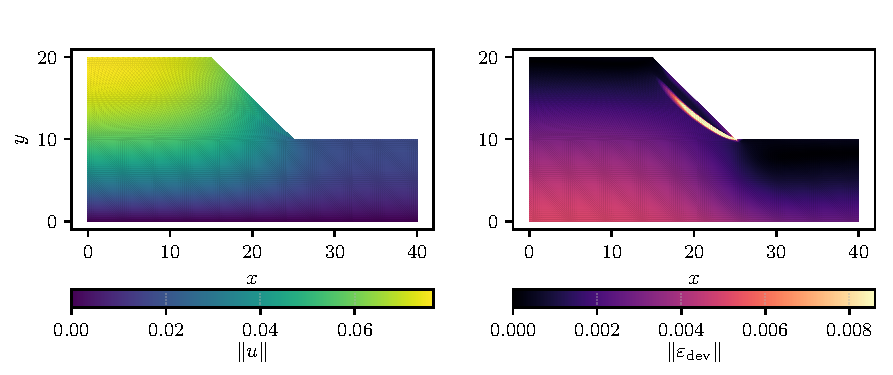
\includegraphics[width=\PaperFigureMedium]{plasticity2d_state_pair.pdf}
  \caption{Representative Plasticity2D state: displacement magnitude and
  deviatoric strain derived from the scalar surrogate
  \cref{eq:plasticity2d-discrete}.}
  \label{fig:plasticity2d-state}
\end{figure}

\begin{figure}[H]
  \centering
  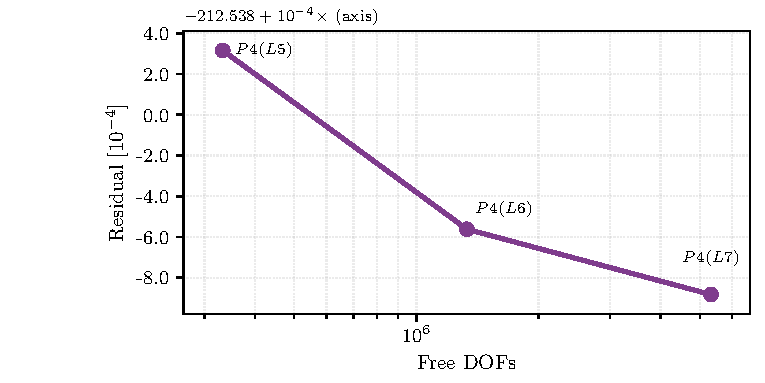
\includegraphics[width=\PaperFigureNarrow]{plasticity2d_resolution_energy.pdf}
  \caption{Resolution trend for the maintained Plasticity2D family. The plotted
  terminal energies are evaluations of \cref{eq:plasticity2d-discrete} on the
  curated $P4(L5)$ showcase and on the larger fixed-work $P4(L6)$ and
  $P4(L7)$ campaigns.}
  \label{fig:plasticity2d-energy-levels}
\end{figure}

\begin{table}[H]
  \centering
  \begin{tabular}{@{}l c c c l@{}}
\toprule
Case & Free DOFs & Energy & Wall time [s] & Note \\
\midrule
$P_{4}(L_{5})$ & \num{332960} & \num{-212.538} & \num{147} & curated showcase \\
$P_{4}(L_{6})$ & \num{1331520} & \num{-212.539} & \num{147} & fixed-work at 8 ranks \\
$P_{4}(L_{7})$ & \num{5325440} & \num{-212.539} & \num{253} & fixed-work at 16 ranks \\
\bottomrule
\end{tabular}

  \caption{Representative Plasticity2D endpoint values from
  \cref{eq:plasticity2d-discrete}.}
  \label{tab:plasticity2d-benchmark}
\end{table}

This family is where multigrid hierarchy design first becomes dominant in the
paper. Solver-engineering evidence for Plasticity2D is reported later in
\Cref{sec:num-plasticity2d,sec:solver-evidence}.

\subsection{Plasticity3D}
\label{sec:bench-plasticity3d}

The literature model is again quasi-static Mohr--Coulomb equilibrium with
constitutive/history updates, now on a three-dimensional heterogeneous slope
geometry
\citep{davis1968plasticity,simo1985consistent,simo1998compinel,tschuchnigg2015nonassociated,sysala2017returnmapping,sysala2025advancedcontinuation}.
The unknown is a displacement field
$u = (u_x,u_y,u_z): \Omega \to \mathbb{R}^3$, gravity acts in the source
$y$-direction. At increment $n+1$, the continuum equilibrium equations are
\begin{equation}
  -\nabla \cdot \sigma^{n+1} = \rho g_y^{n+1} e_y
  \quad \text{in }\Omega,
  \qquad
  u_i^{n+1} = \bar u_i^{n+1} \quad \text{on }\Gamma_{D,i},
  \qquad
  \sigma^{n+1}n = 0 \quad \text{on }\Gamma_N,
  \label{eq:plasticity3d-strong}
\end{equation}
where $\sigma^{n+1}$ and the internal variables are obtained from the
elastoplastic update driven by $\varepsilon(u^{n+1})$ and the previous state.
The corresponding weak form is
\begin{equation}
  \int_{\Omega} \sigma^{n+1} : \varepsilon(v) \, dx
  =
  \int_{\Omega} \rho g_y^{n+1} e_y \cdot v \, dx
  \qquad \forall v \in V_0.
  \label{eq:plasticity3d-weak}
\end{equation}
The repository specialization studied in this paper uses the imported SSR mesh
hierarchy with same-mesh tetrahedral $P1/P2/P4$ spaces, source component-wise
boundary labels, and an additional glued-bottom condition that fixes every node
with $|y| \le 10^{-12}$ in all three displacement components. The benchmark-local
figures below use the corrected glued-bottom $\code{P4(L1\_2)}$ showcase at
$\lambda_{\mathrm{sr}}=1.55$ and the finished nine-case maintained-local study
at the same load factor. The promoted $\lambda_{\mathrm{sr}}=1.0$ strong-scaling
campaign is kept later in the paper as separate historical timing evidence.
For those endpoint and continuation studies, the maintained code evaluates the
following algorithmic scalar surrogate:
\begin{equation}
  \Pi_h^{3\mathrm{D}}(u_h;\lambda_{\mathrm{sr}})
  =
  \sum_{e=1}^{n_{\mathrm{el}}}
  \sum_{q=1}^{n_q}
    w_{eq}\,
    \Phi_{\mathrm{MC},3\mathrm{D}}
    \!\left(
      \varepsilon_{eq}(u_e),
      \bar c_{\lambda,eq},
      \sin \phi_{\lambda,eq},
      \mu_{eq},
      K_{eq},
      \lambda_{\mathrm{L},eq}
    \right)
  - f_{\mathrm{ext}}^T u_h,
  \label{eq:plasticity3d-discrete}
\end{equation}
where $\lambda_{\mathrm{sr}}$ is again the strength-reduction factor and
$\lambda_{\mathrm{L}}$ is the Lam{\'e} parameter of the elastic predictor.

The code uses the engineering-strain ordering
\begin{equation}
  \varepsilon
  =
  \begin{bmatrix}
    \varepsilon_{xx} &
    \varepsilon_{yy} &
    \varepsilon_{zz} &
    \gamma_{xy} &
    \gamma_{yz} &
    \gamma_{xz}
  \end{bmatrix}^{T},
  \label{eq:plasticity3d-engineering-strain}
\end{equation}
which is first mapped to tensor shear before principal values are formed. The
benchmark keeps the Davis-B reduction explicitly at quadrature points:
\begin{align}
  c_{1,q} &= c_{0,q}/\lambda_{\mathrm{sr}},
  &
  \phi_{1,q} &= \arctan\!\left(\tan\phi_q/\lambda_{\mathrm{sr}}\right),
  &
  \psi_{1,q} &= \arctan\!\left(\tan\psi_q/\lambda_{\mathrm{sr}}\right),
  \nonumber\\
  \beta_q &= \frac{\cos\phi_{1,q}\cos\psi_{1,q}}
                 {1-\sin\phi_{1,q}\sin\psi_{1,q}},
  &
  c_{\lambda,q} &= \beta_q c_{1,q},
  &
  \phi_{\lambda,q} &= \arctan\!\left(\beta_q \tan\phi_{1,q}\right),
  \label{eq:plasticity3d-davis}
\end{align}
with
\begin{equation}
  \bar c_{\lambda,q} = 2 c_{\lambda,q}\cos\phi_{\lambda,q},
  \qquad
  \sin\phi_{\lambda,q} = \sin(\phi_{\lambda,q}),
  \label{eq:plasticity3d-davis-bar}
\end{equation}
which are the scalar constitutive parameters actually stored in the maintained
3D assembly path
\citep{davis1968plasticity,tschuchnigg2015nonassociated,sysala2021optimization}.
Here $\phi$ denotes friction angle and $\psi$ denotes dilation angle; the paper
uses those symbols only in that geomechanics sense.

The local constitutive surrogate follows the piecewise branch structure used in
the repository. Let $\varepsilon_1 \ge \varepsilon_2 \ge \varepsilon_3$ be the
principal strains and let
\begin{equation}
  I_1 = \varepsilon_{xx} + \varepsilon_{yy} + \varepsilon_{zz},
  \qquad
  q(\varepsilon) =
  \varepsilon_{xx}^2 + \varepsilon_{yy}^2 + \varepsilon_{zz}^2
  + \frac{1}{2}\left(
    \gamma_{xy}^2 + \gamma_{yz}^2 + \gamma_{xz}^2
  \right).
  \label{eq:plasticity3d-invariants}
\end{equation}
The elastic branch is
\begin{equation}
  \Phi_{\mathrm{el}}
  = \frac{1}{2}\lambda_{\mathrm{L}} I_1^2 + \mu q(\varepsilon),
  \label{eq:plasticity3d-elastic-branch}
\end{equation}
and the source-style return variables are
\begin{align}
  f_{\mathrm{tr}}
  &=
  2\mu\!\left((1+\sin\phi_{\lambda})\varepsilon_1 -
  (1-\sin\phi_{\lambda})\varepsilon_3\right)
  + 2\lambda_{\mathrm{L}}\sin\phi_{\lambda} I_1
  - \bar c_{\lambda},
  \nonumber\\
  \gamma_{\mathrm{sl}}
  &= \frac{\varepsilon_1-\varepsilon_2}{1+\sin\phi_{\lambda}},
  \qquad
  \gamma_{\mathrm{sr}}
  = \frac{\varepsilon_2-\varepsilon_3}{1-\sin\phi_{\lambda}},
  \label{eq:plasticity3d-return-tests}
\end{align}
with the remaining left, right, and apex thresholds defined as in the code
through the same principal-strain ordering. The scalar potential is then the
piecewise function
\begin{equation}
  \Phi_{\mathrm{MC},3\mathrm{D}}
  =
  \begin{cases}
    \Phi_{\mathrm{el}},
      & f_{\mathrm{tr}} \le 0, \\
    \Phi_{\mathrm{s}},
      & \Lambda_{\mathrm{s}} \le \min(\gamma_{\mathrm{sl}},\gamma_{\mathrm{sr}}), \\
    \Phi_{\mathrm{l}},
      & \gamma_{\mathrm{sl}} < \gamma_{\mathrm{sr}}
        \text{ and }
        \gamma_{\mathrm{sl}} \le \Lambda_{\mathrm{l}} \le \gamma_{\mathrm{la}}, \\
    \Phi_{\mathrm{r}},
      & \gamma_{\mathrm{sr}} < \gamma_{\mathrm{sl}}
        \text{ and }
        \gamma_{\mathrm{sr}} \le \Lambda_{\mathrm{r}} \le \gamma_{\mathrm{ra}}, \\
    \Phi_{\mathrm{a}},
      & \text{otherwise},
  \end{cases}
  \label{eq:plasticity3d-potential}
\end{equation}
where the branch energies $\Phi_{\mathrm{s}}$, $\Phi_{\mathrm{l}}$,
$\Phi_{\mathrm{r}}$, and $\Phi_{\mathrm{a}}$ are the repository's branchwise
quadratic corrections to \cref{eq:plasticity3d-elastic-branch}. The maintained
constitutive-AD path differentiates the smooth branches of
\cref{eq:plasticity3d-potential} directly with JAX rather than substituting a
hand-derived return-map tangent; the branch interfaces remain nonsmooth and are
treated as part of the algorithmic constitutive surrogate rather than as a
globally smooth continuum potential.

For the strain visualizations in this paper we use the deviatoric norm
\begin{equation}
  \|\varepsilon_{\mathrm{dev}}\|
  =
  \sqrt{
    \varepsilon^T
    \left(
      \operatorname{diag}(1,1,1,\tfrac{1}{2},\tfrac{1}{2},\tfrac{1}{2})
      - \frac{1}{3}mm^T
    \right)
    \varepsilon
  },
  \qquad
  m = (1,1,1,0,0,0)^T,
  \label{eq:plasticity3d-devnorm}
\end{equation}
which matches the engineering-shear convention of
\cref{eq:plasticity3d-engineering-strain}.

Because \cref{eq:plasticity3d-discrete,eq:plasticity3d-potential} define an
algorithmic endpoint surrogate rather than a path-consistent incremental
history functional, the results section reports this family with a separate
validation ladder. Same-case source-faithfulness to the source-style surrogate
implementation is treated separately from a fixed-lambda source-operator
comparison. The latter checks source-family behavior under matched geometry,
materials, boundary constraints, and reduction parameters, but it is not a
path-consistent incremental-history validation. The paper therefore keeps the
Plasticity3D claims at the level of a repository-specific surrogate
approximation rather than a path-consistent replacement. The related
convex-optimization and continuation literature
\citep{sysala2025convexoptimization,sysala2025advancedcontinuation} is used as
source-family context, not as evidence that this repository surrogate is a full
incremental elastoplastic solver.

\begin{figure}[H]
  \centering
  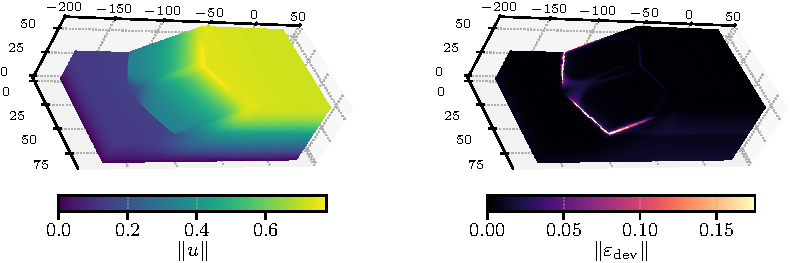
\includegraphics[width=\PaperFigureMedium]{plasticity3d_state_pair.pdf}
  \caption{Corrected glued-bottom Plasticity3D showcase at
  $\lambda_{\mathrm{sr}}=1.55$: displacement magnitude and surface deviatoric
  strain for the maintained-local \code{P4(L1\_2)} run, both derived from the
  scalar surrogate in
  \cref{eq:plasticity3d-discrete}.}
  \label{fig:plasticity3d-state}
\end{figure}

\begin{figure}[H]
  \centering
  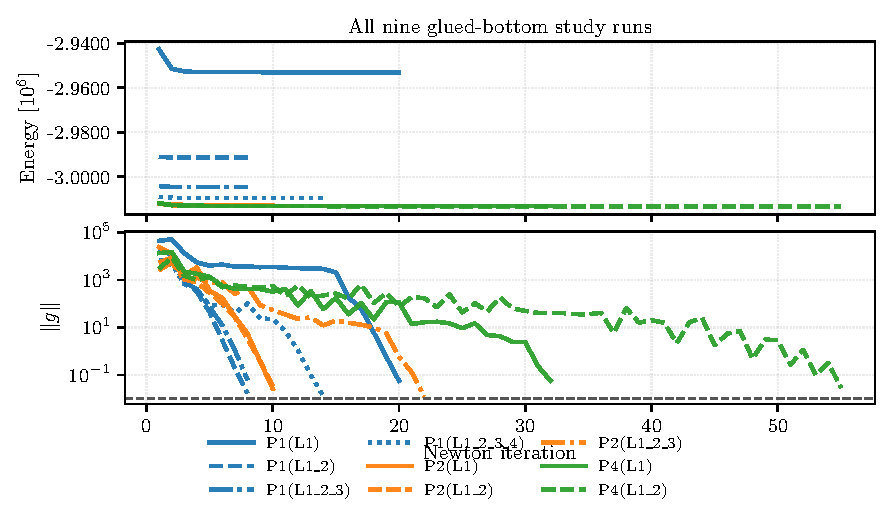
\includegraphics[width=\PaperFigureMedium]{plasticity3d_convergence.pdf}
  \caption{Newton-history convergence for all nine completed corrected
  glued-bottom maintained-local Plasticity3D study runs at
  $\lambda_{\mathrm{sr}}=1.55$. The upper panel shows the value of the
  algorithmic surrogate from \cref{eq:plasticity3d-discrete}; the lower panel
  shows the gradient norm used as the nonlinear stopping metric, with color
  indicating degree and line style indicating mesh level.}
  \label{fig:plasticity3d-convergence}
\end{figure}

\begin{table}[H]
  \centering
  \begin{tabular*}{\textwidth}{@{}l@{\extracolsep{\fill}} c c c c@{}}
\toprule
Element & Free DOFs & Energy & $\|g\|_{\mathrm{final}}$ & Wall time [s] \\
\midrule
$P_{1}(L_{1})$ & \num{10526} & \num{-2953167} & $\num{4.56}\times 10^{-3}$ & \num{1.79} \\
$P_{1}(L_{2})$ & \num{79024} & \num{-2991497} & $\num{1.64}\times 10^{-3}$ & \num{8.72} \\
$P_{1}(L_{3})$ & \num{610964} & \num{-3004742} & $\num{4.07}\times 10^{-3}$ & \num{17.2} \\
$P_{1}(L_{4})$ & \num{4801816} & \num{-3009658} & $\num{1.16}\times 10^{-3}$ & \num{96.7} \\
$P_{2}(L_{1})$ & \num{79024} & \num{-3012813} & $\num{2.47}\times 10^{-3}$ & \num{18.3} \\
$P_{2}(L_{2})$ & \num{610964} & \num{-3013032} & $\num{2.96}\times 10^{-3}$ & \num{98.3} \\
$P_{2}(L_{3})$ & \num{4801816} & \num{-3013149} & $\num{1.14}\times 10^{-3}$ & \num{1330} \\
$P_{4}(L_{1})$ & \num{610964} & \num{-3013227} & $\num{5.53}\times 10^{-3}$ & \num{208} \\
$P_{4}(L_{2})$ & \num{4801816} & \num{-3013348} & $\num{4.42}\times 10^{-3}$ & \num{2298} \\
\bottomrule
\end{tabular*}

  \caption{All nine completed glued-bottom maintained-local Plasticity3D
  study rows at $\lambda_{\mathrm{sr}} = 1.55$, reported as endpoint values of
  \cref{eq:plasticity3d-discrete}.}
  \label{tab:plasticity3d-benchmark}
\end{table}

\begin{figure}[H]
  \centering
  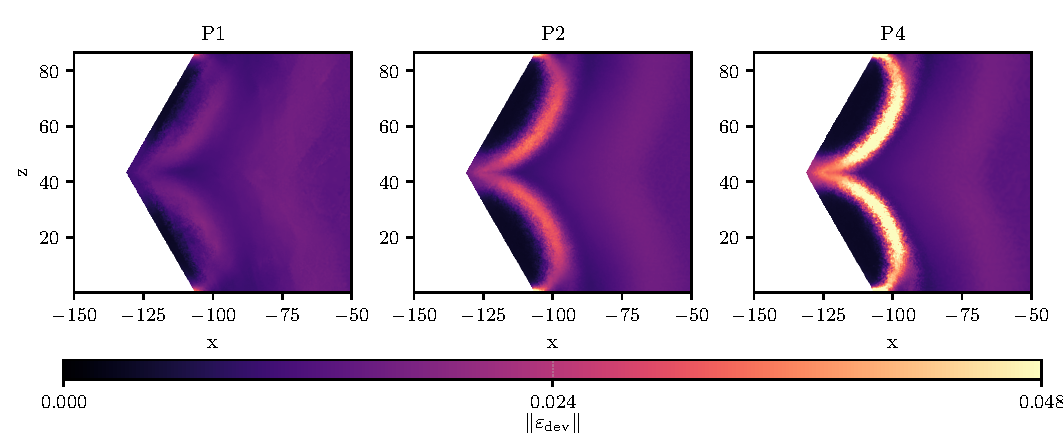
\includegraphics[width=\PaperFigureFull]{plasticity3d_highest_mesh_y_slice_comparison.pdf}
  \caption{Shared-scale upper $y$-slice comparison of
  $\|\varepsilon_{\mathrm{dev}}\|$ from \cref{eq:plasticity3d-devnorm} at the
  highest mesh level of each degree line:
  \code{P1(L1\_2\_3\_4)}, \code{P2(L1\_2\_3)}, and \code{P4(L1\_2)}. The three
  runs use the corrected glued-bottom maintained-local solver stack at
  $\lambda_{\mathrm{sr}} = 1.55$ and are compared on one common color scale.}
  \label{fig:plasticity3d-highest-slice}
\end{figure}

Plasticity3D is the benchmark where detailed constitutive definitions are most
important: the paper later plots values of \cref{eq:plasticity3d-discrete} and
\cref{eq:plasticity3d-devnorm}, so both quantities are defined explicitly here.
Timing, scaling, and degree-versus-resolution evidence for this family are
reported in \Cref{sec:num-plasticity3d}.

\subsection{Topology Optimization}
\label{sec:bench-topology}

The literature model is the standard SIMP-style compliance topology-optimization
setting on a cantilever domain, together with filtering and continuation ideas
from the classical topology literature
\citep{bendsoe2003topology,sigmund2001topology,ferrari2020top99,bourdin2001filters}.
In the repository specialization studied here, the topology benchmark is a
reduced optimization problem rather than a single equilibrium minimization. The
design variable is a latent nodal field
$z_h \in Z_h$, mapped to a physical density through the logistic transform
\begin{equation}
  \theta_h(z_h)
  =
  \theta_{\min} + (1-\theta_{\min}) \sigma(z_h),
  \qquad
  \sigma(z) = \frac{1}{1+e^{-z}}.
  \label{eq:topology-density-map}
\end{equation}
For fixed density, the maintained discretization solves for the linear elastic
displacement state
$u_h(\theta_h)$ solving
\begin{equation}
  a_{\theta_h}(u_h,v_h)
  :=
  \sum_{e=1}^{n_{\mathrm{el}}}
    |e|\,\theta_e^{p}
    \varepsilon(u_h)^T C \varepsilon(v_h)
  =
  \ell(v_h)
  \qquad \forall v_h \in V_{h,0},
  \label{eq:topology-mechanics}
\end{equation}
on the cantilever domain $\Omega = (0,2)\times(0,1)$ with clamped left edge
and prescribed traction on a right-edge patch. The reduced objective solved in
the maintained code is
\begin{align}
  \mathcal{J}_h(z_h)
  &=
  \sum_{e=1}^{n_{\mathrm{el}}}
  |e|
  \Bigg[
    e_e^{\mathrm{frozen}} \theta_e^{-p}
    + \lambda_V \theta_e
    + \alpha_{\mathrm{reg}}
      \left(
        \frac{\ell_{\mathrm{pf}}}{2} \lvert \nabla \theta_e \rvert^2
        + \frac{1}{\ell_{\mathrm{pf}}} W(\theta_e)
      \right)
    + \frac{\mu_{\mathrm{move}}}{2} (z_e-z_e^{\mathrm{old}})^2
  \Bigg],
  \label{eq:topology-reduced-objective}
\end{align}
with $W(\theta) = \theta^2(1-\theta)^2$, SIMP-style continuation in $p$, and
repository regularization terms that play a mesh-control role analogous to
filtering/regularization in \citet{bourdin2001filters}. Here
$e_e^{\mathrm{frozen}}$ denotes the element elastic energy density from the
previous mechanics state; the latent logistic map, frozen-energy term, and move
penalty are repository-specific design choices rather than standard SIMP
notation. The maintained outer loop alternates mechanics solves for
\cref{eq:topology-mechanics} with reduced design updates for
\cref{eq:topology-reduced-objective}.

\begin{figure}[H]
  \centering
  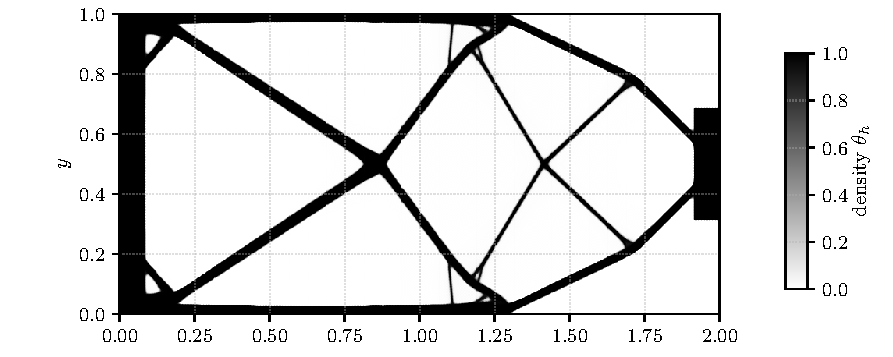
\includegraphics[width=\PaperFigureMedium]{topology_density.pdf}
  \caption{Representative final density field for the maintained parallel
  topology benchmark.}
  \label{fig:topology-density}
\end{figure}

\begin{figure}[H]
  \centering
  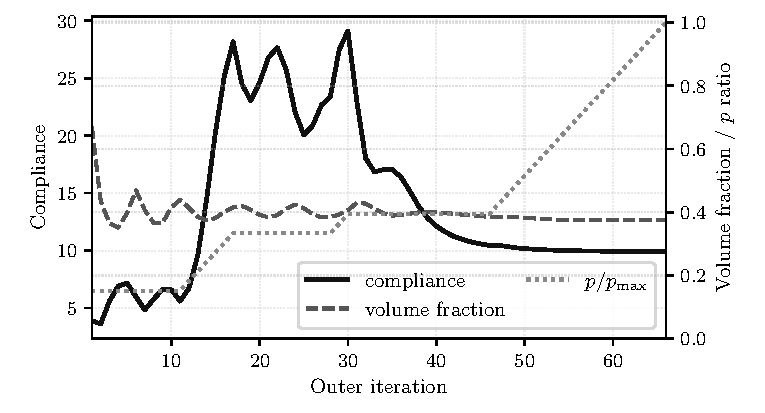
\includegraphics[width=0.96\PaperFigureNarrow]{topology_history.pdf}
  \caption{Objective-history view for the reduced topology objective
  \cref{eq:topology-reduced-objective}, with compliance on the left axis and
  volume fraction plus the continuation schedule in $p$ on the right axis.}
  \label{fig:topology-history}
\end{figure}

\begin{table}[H]
  \centering
  \begin{tabular*}{\textwidth}{@{}l@{\extracolsep{\fill}} c c c c c@{}}
\toprule
Case & Ranks & Outer iters & Compliance & Volume fraction & Wall time [s] \\
\midrule
192$\times$96 & 1 & 121 & \num{4.1557} & \num{0.4} & \num{10} \\
768$\times$384 & 32 & 66 & \num{9.9074} & \num{0.3749} & \num{25.1} \\
\bottomrule
\end{tabular*}

  \caption{Representative topology endpoint values from
  \cref{eq:topology-reduced-objective}.}
  \label{tab:topology-benchmark}
\end{table}

For topology, the relevant notion of ``convergence'' is the reduced objective
history rather than a single equilibrium energy. Parallel timing and scaling
for the same family are reported in \Cref{sec:num-topology}.


\section{Numerical Examples}
\label{sec:numerical-examples}

This section turns from problem definition to computational behavior. The
benchmark families in \Cref{sec:benchmarks} established the governing
equations, discrete energies, and representative states, and
\Cref{sec:validation} separated the validation and external-comparison
evidence. Here we focus on parallel timings, scaling trends, solver behavior,
and the comparative cost of alternative derivative or discretization choices.
Evidence from older timing studies is retained when it is still informative for
workflow viability, but it is labeled as timing evidence rather than merged into
the validation story.

\subsection{\texorpdfstring{$p$-Laplace}{p-Laplace}}
\label{sec:num-plaplace}

The $p$-Laplace problem definition and discrete energy are given in
\Cref{sec:bench-plaplace,eq:plaplace-discrete}. In this clean scalar setting,
the numerical story is easiest to interpret: exact element Hessians remain
effective in the reported distributed runs, while local-SFD reaches nearly
identical discrete energies at higher wall time.

\begin{figure}[H]
  \centering
  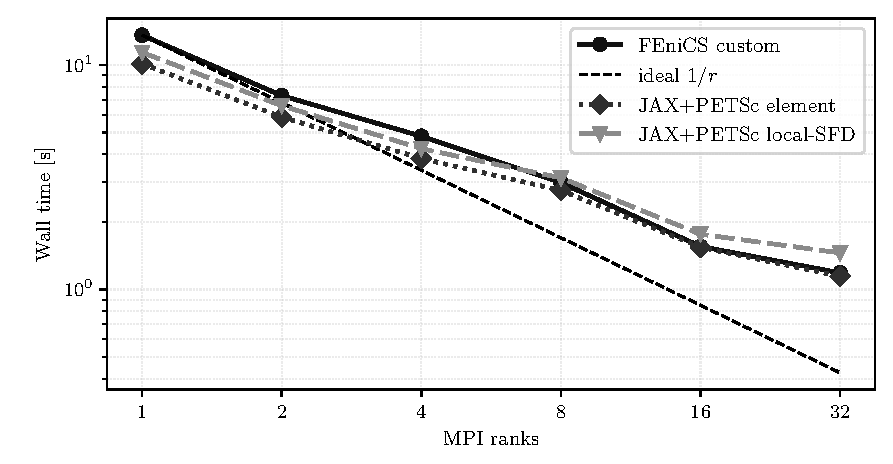
\includegraphics[width=\PaperFigureMedium]{plaplace_scaling.pdf}
  \caption{$p$-Laplace strong scaling on the finest maintained grid. All curves
  correspond to the same discrete problem from \cref{eq:plaplace-discrete}.}
  \label{fig:plaplace-results}
\end{figure}

\subsection{Ginzburg--Landau}
\label{sec:num-gl}

The Ginzburg--Landau family from \Cref{sec:bench-gl,eq:gl-discrete} shows the
same high-level derivative story under a more indefinite linearization. The
important computational message is not a dramatic separation between exact and
approximate second-order routes, but that the maintained distributed solver
remains convergent on this nonconvex scalar energy with the same sparse-infrastructure
contract.

\begin{figure}[H]
  \centering
  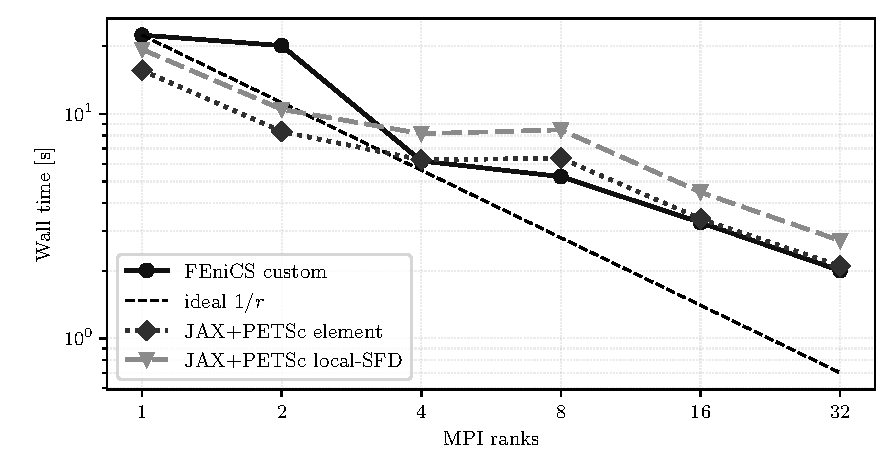
\includegraphics[width=\PaperFigureMedium]{ginzburg_landau_scaling.pdf}
  \caption{Ginzburg--Landau strong scaling for the maintained fine-grid case
  governed by \cref{eq:gl-discrete}.}
  \label{fig:gl-results}
\end{figure}

\subsection{Hyperelasticity}
\label{sec:num-hyperelasticity}

The hyperelasticity problem definition, boundary data, and terminal energies
are given in \Cref{sec:bench-he,eq:hyperelasticity-discrete}. Computationally,
this is the maintained benchmark in which globalization matters more than
derivative-route choice: the distributed implementation completes the full load
path and preserves the terminal energy trend from \Cref{sec:bench-he}. The
external JAX-FEM companion comparison is reported separately in
\Cref{sec:val-hyperelasticity}; the figure below reports only distributed
scaling for the repository load path.

\begin{figure}[H]
  \centering
  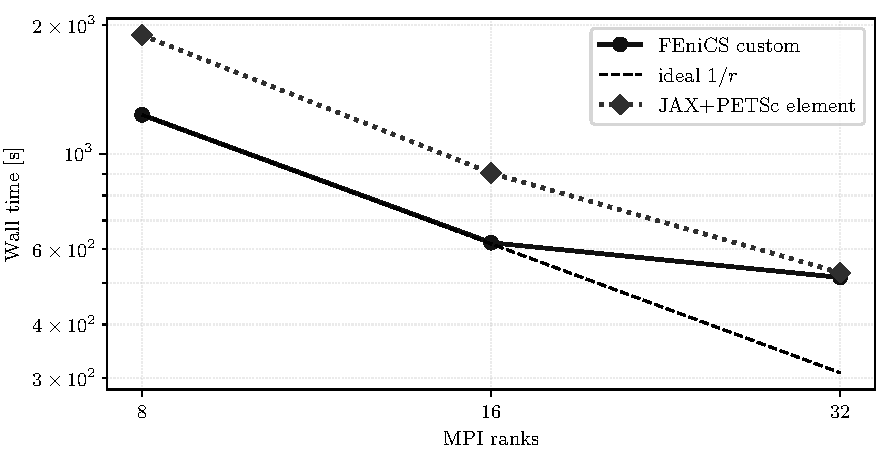
\includegraphics[width=\PaperFigureMedium]{hyperelasticity_scaling.pdf}
  \caption{Hyperelasticity strong scaling for the 24-step load path defined by
  \cref{eq:hyperelasticity-discrete}.}
  \label{fig:hyperelasticity-results}
\end{figure}

The larger fixed-work Karolina experiment isolates the first level-5 load
step after the rank-local HyperElasticity implementation. The Karolina CPU
nodes used here are IT4I standard CPU nodes with two AMD EPYC 7H12 64-core
processors and 256 GB RAM \citep{it4i-karolina-compute-nodes}; on the tested
nodes Slurm exposes the 128 cores as eight NUMA domains with 16 cores each.
The runs use one MPI rank per core, contiguous CPU-ID binding, and local memory
binding. The mesh is generated procedurally from the uniform beam hierarchy,
and the element path assembles from rank-local elements with local PETSc COO
preallocation and point-to-point overlap exchange.

The nonlinear solve is the same trust-region Newton path used for the
benchmark in \cref{sec:bench-he}. The linear subproblems use STCG with a
same-hierarchy PMG preconditioner, Chebyshev/Jacobi smoothing, and coarsest
level $L_2$. The coarse solve is PETSc redundant LU with MUMPS: the partial
one-node rows use one redundant group over the active ranks, while the
multi-node rows use one 128-rank redundant group per node.
\Cref{fig:hyperelasticity-karolina-pmg-scaling,tab:hyperelasticity-karolina-pmg-scaling}
report the application-reported solver total time, not Slurm elapsed time.
All rows reach the same first-step energy to the precision shown in the raw
outputs, with 21 Newton iterations and 43 Krylov iterations.

\begin{figure}[H]
  \centering
  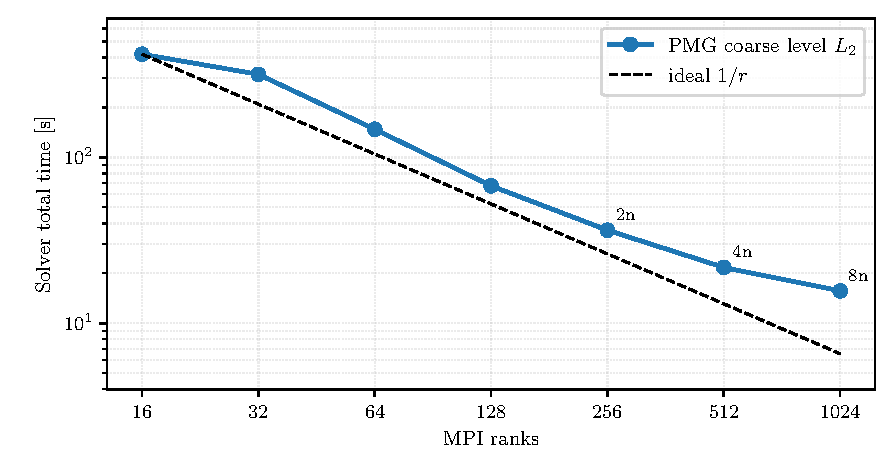
\includegraphics[width=\PaperFigureMedium]{hyperelasticity_karolina_pmg_scaling.pdf}
  \caption{Karolina level-5 HyperElasticity first-step fixed-work scaling with
  the PMG coarse level fixed at $L_2$. Multi-node annotations show node counts.}
  \label{fig:hyperelasticity-karolina-pmg-scaling}
\end{figure}

\begin{table}[H]
  \centering
  \begin{tabular*}{\textwidth}{@{}c@{\extracolsep{\fill}} c c c c c c c@{}}
\toprule
Ranks & Nodes & Coarse groups & Ranks/group & Solver total [s] & First step [s] & Newton iters & Krylov iters \\
\midrule
16 & 1 & 1 & 16 & \num{419} & \num{367} & 21 & 43 \\
32 & 1 & 1 & 32 & \num{317} & \num{280} & 21 & 43 \\
64 & 1 & 1 & 64 & \num{148} & \num{132} & 21 & 43 \\
128 & 1 & 1 & 128 & \num{67.4} & \num{58.4} & 21 & 43 \\
256 & 2 & 2 & 128 & \num{36.4} & \num{30.7} & 21 & 43 \\
512 & 4 & 4 & 128 & \num{21.7} & \num{17.7} & 21 & 43 \\
1024 & 8 & 8 & 128 & \num{15.7} & \num{12.3} & 21 & 43 \\
\bottomrule
\end{tabular*}

  \caption{Karolina level-5 HyperElasticity first-step timings used in
  \cref{fig:hyperelasticity-karolina-pmg-scaling}.}
  \label{tab:hyperelasticity-karolina-pmg-scaling}
\end{table}

\subsection{Plasticity2D}
\label{sec:num-plasticity2d}

The Plasticity2D model and Davis-B reduction are defined in
\Cref{sec:bench-plasticity2d,eq:plasticity2d-discrete,eq:plasticity2d-davis}.
For this family, the most informative computational evidence is not a single
strong-scaling curve but the solver-engineering material collected in
\Cref{sec:solver-evidence}: same-mesh PMG choices, fixed-work runs, and source
continuation behavior. We therefore keep the within-benchmark resolution trend
in \Cref{fig:plasticity2d-energy-levels} and defer the supporting solver data
to the later evidence section.

\subsection{Plasticity3D}
\label{sec:num-plasticity3d}

The governing problem, Davis-B reduction, scalar constitutive potential, and
deviatoric-strain norm are defined in
\Cref{sec:bench-plasticity3d,eq:plasticity3d-discrete,eq:plasticity3d-davis,eq:plasticity3d-potential,eq:plasticity3d-devnorm}.
The validation limits for this endpoint surrogate are reported in
\Cref{sec:val-plasticity3d}. With that interpretation fixed, this section asks
two performance questions: which second-order route is preferred on the locked
flagship case, and how the maintained surrogate behaves across degree,
resolution, and rank count.

\paragraph{Derivative-route ablation.}
The first question is which second-order route has the most useful
cost-quality profile for the promoted maintained workflow. On the locked
$P_4(L_1)$ case at $\lambda_{\mathrm{sr}}=1.5$ and 8 MPI ranks, all three
routes converge to essentially the same terminal state, with identical Newton
and total Krylov counts. The differences are therefore cost differences, not
state-quality differences: constitutive AD has the lowest median wall time on
this locked case, with median wall time \SI{222}{s} and median solve time
\SI{191}{s}, compared with \SI{288}{s}/\SI{255}{s} for element AD
and \SI{372}{s}/\SI{253}{s} for colored SFD.

\begin{figure}[H]
  \centering
  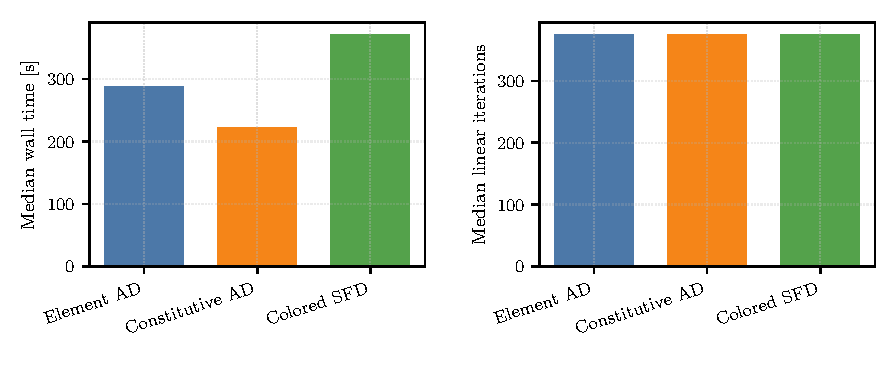
\includegraphics[width=\PaperFigureMedium]{plasticity3d_derivative_ablation_bars.pdf}
  \caption{Locked Plasticity3D derivative-route ablation on
  $P_4(L_1)$, $\lambda_{\mathrm{sr}}=1.5$, and 8 MPI ranks.}
  \label{fig:plasticity3d-derivative-ablation}
\end{figure}

\begin{table}[H]
  \centering
  \begin{tabularx}{\textwidth}{@{}>{\hsize=0.88\hsize\linewidth=\hsize\RaggedRight\arraybackslash}Xr r r r r r r@{}}
\toprule
Route & Wall [s] & Solve [s] & Newton & Linear & Energy & $\omega$ & $u_{\max}$ \\
\midrule
Element AD & 288.021 & 254.879 & 8.00 & 376.0 & -3010860.766733 & 6027722.264408 & 0.731848 \\
Constitutive AD & 221.689 & 190.503 & 8.00 & 376.0 & -3010860.766439 & 6027722.229618 & 0.731848 \\
Colored SFD & 371.993 & 252.814 & 8.00 & 376.0 & -3010860.766733 & 6027722.264408 & 0.731848 \\
\bottomrule
\end{tabularx}

  \caption{Plasticity3D derivative-route ablation on the locked
  $P_4(L_1)$, $\lambda_{\mathrm{sr}}=1.5$, 8-rank case.}
  \label{tab:plasticity3d-derivative-ablation}
\end{table}

\paragraph{Maintained discretization and historical scaling.}
The remaining figures in this subsection answer a different question: how the
maintained surrogate behaves across degree/resolution choices, and how the
recommended maintained stack scales on the separate promoted
$P_4(L_2)$ timing study.

\begin{figure}[H]
  \centering
  \begin{subfigure}[t]{0.46\PaperFigureFull}
    \centering
    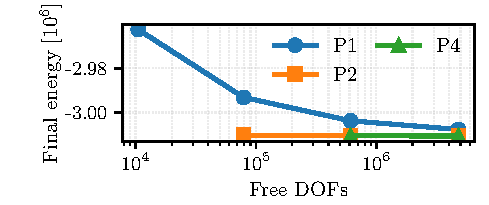
\includegraphics[width=\linewidth]{plasticity3d_degree_energy_all_dofs.pdf}
    \caption{All degrees: final energy versus free DOFs.}
  \end{subfigure}
  \hfill
  \begin{subfigure}[t]{0.46\PaperFigureFull}
    \centering
    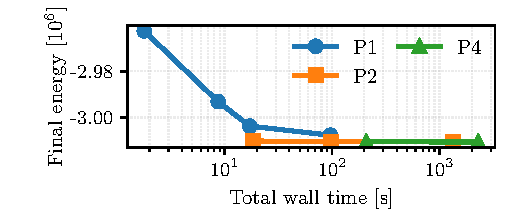
\includegraphics[width=\linewidth]{plasticity3d_degree_energy_all_time.pdf}
    \caption{All degrees: final energy versus total wall time.}
  \end{subfigure}

  \vspace{0.45em}

  \begin{subfigure}[t]{0.46\PaperFigureFull}
    \centering
    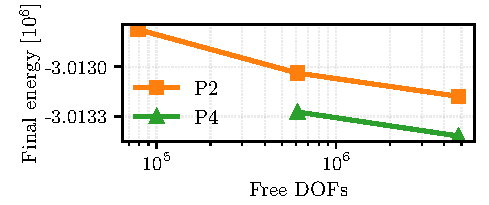
\includegraphics[width=\linewidth]{plasticity3d_degree_energy_zoom_dofs.pdf}
    \caption{$P2/P4$ zoom: final energy versus free DOFs.}
  \end{subfigure}
  \hfill
  \begin{subfigure}[t]{0.46\PaperFigureFull}
    \centering
    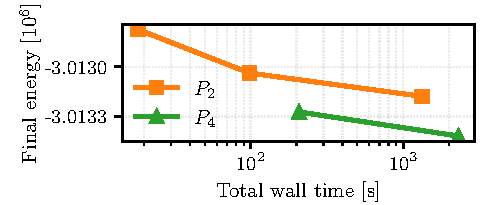
\includegraphics[width=\linewidth]{plasticity3d_degree_energy_zoom_time.pdf}
    \caption{$P2/P4$ zoom: final energy versus total wall time.}
  \end{subfigure}
  \caption{Corrected glued-bottom maintained Plasticity3D
  degree-versus-resolution study at $\lambda_{\mathrm{sr}} = 1.55$. The top
  row shows the full $P_1/P_2/P_4$ comparison, while the bottom row zooms to
  $P_2/P_4$ so the near-overlap hidden by the coarse $P_1$ points becomes
  visible. The left column plots final values of
  \cref{eq:plasticity3d-discrete} against free DOFs; the right column plots
  the same converged energies against end-to-end wall time. All timings are
  fair 32-rank maintained runs.}
  \label{fig:plasticity3d-degree-energy}
\end{figure}

The zoom row in \Cref{fig:plasticity3d-degree-energy} is essential because the
full figure is dominated by coarse $P_1$ variation. Under the corrected
glued-bottom constraint, the first matched comparison is
$P_4(L_1)$ versus $P_1(L_3)$ at \num{610964} free DOFs. The second
matched comparison is $P_1(L_4)$, $P_2(L_3)$, and $P_4(L_2)$ at
\num{4801816} free DOFs. The scientific message is
therefore that the maintained solver reaches similar terminal energies along
both $p$- and $h$-refined paths, while higher order on coarser meshes buys
lower energy at matched DOFs only by paying a clear wall-time premium.

\begin{figure}[H]
  \centering
  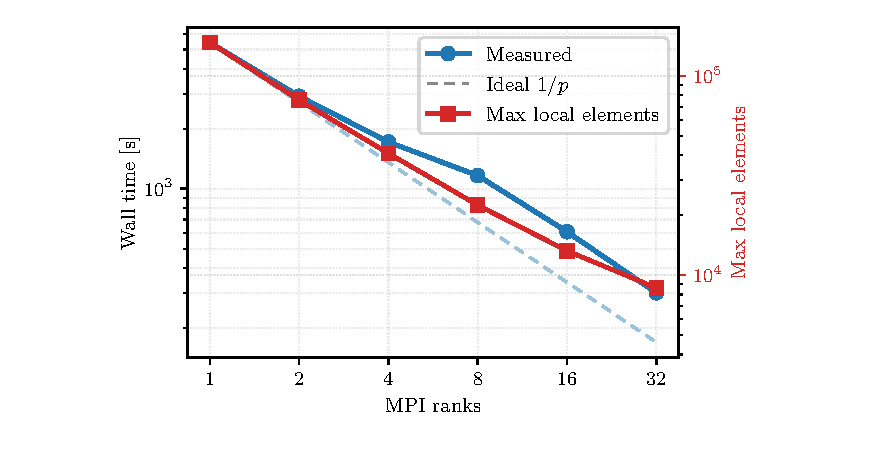
\includegraphics[width=\PaperFigureMedium]{plasticity3d_recommended_scaling.pdf}
  \caption{Historical strong scaling for the promoted Plasticity3D maintained
  stack: \localpmg{} on $P_4(L_2)$ at
  $\lambda_{\mathrm{sr}} = 1.0$. This is a separate timing study from the
  glued-bottom $\lambda_{\mathrm{sr}} = 1.55$ results shown in
  \cref{fig:plasticity3d-state,fig:plasticity3d-convergence,fig:plasticity3d-degree-energy}.}
  \label{fig:plasticity3d-scaling}
\end{figure}

\begin{table}[H]
  \centering
  \begin{tabular*}{\textwidth}{@{}c@{\extracolsep{\fill}} c c c c c c@{}}
\toprule
Ranks & Wall time [s] & Solve time [s] & Speedup & Efficiency & Newton iters & Krylov iters \\
\midrule
1 & \num{5424} & \num{5176} & \num{1} & \num{1} & 17 & 114 \\
2 & \num{2914} & \num{2777} & \num{1.861} & \num{0.931} & 17 & 114 \\
4 & \num{1717} & \num{1634} & \num{3.16} & \num{0.79} & 17 & 114 \\
8 & \num{1164} & \num{1107} & \num{4.658} & \num{0.582} & 17 & 114 \\
16 & \num{608} & \num{575} & \num{8.916} & \num{0.557} & 17 & 114 \\
32 & \num{300} & \num{284} & \num{18.053} & \num{0.564} & 17 & 114 \\
\bottomrule
\end{tabular*}

  \caption{Historical Plasticity3D strong scaling for \localpmg{} on
  $P_4(L_2)$ at $\lambda_{\mathrm{sr}} = 1.0$. These rows are useful as
  solver evidence, but they should not be read as a direct timing continuation
  of the glued-bottom $\lambda_{\mathrm{sr}} = 1.55$ benchmark figures.}
  \label{tab:plasticity3d-scaling}
\end{table}

\Cref{fig:plasticity3d-scaling,tab:plasticity3d-scaling} give the paper's
largest maintained distributed mechanics timing result. This scaling evidence uses
the promoted $P_4(L_2)$ mesh family but a different load factor,
$\lambda_{\mathrm{sr}} = 1.0$, so it complements rather than extends the
glued-bottom $\lambda_{\mathrm{sr}} = 1.55$ benchmark figures above. Within
that timing study, the reported nonlinear and linear iteration counts
remain matched on 1/2/4/8/16/32 ranks, while the end-to-end time drops from
\SI{5424}{s} on one rank to \SI{300}{s} on 32 ranks. Additional
source-vs-local and continuation evidence is reported later in
\Cref{sec:solver-evidence}.

A final fixed-work diagnostic repeats the glued-bottom
$P_4(L_2)$, $\lambda_{\mathrm{sr}}=\num{1.55}$ case with the current
constitutive-AD local assembly and MUMPS-backed PMG stack. The PMG hierarchy is
the same-mesh $P_4 \rightarrow P_2 \rightarrow P_1$ hierarchy, the nonlinear
method is Armijo Newton, and the Krylov tolerance is \num{1e-1}. Each run is
intentionally capped after five Newton iterations, so the raw solver status is
``maximum number of iterations reached'' even though the fixed work is matched.
\Cref{fig:plasticity3d-local-karolina-scaling,tab:plasticity3d-local-karolina-scaling}
overlay the local workstation sweep with the Karolina CPU-node sweep at
16 MPI ranks per node. All plotted rows use 29 Krylov iterations and reach the
same capped-state energy and gradient norm to the precision shown in the table;
the figure is therefore a fixed-work implementation diagnostic rather than a
new convergence claim.

\begin{figure}[H]
  \centering
  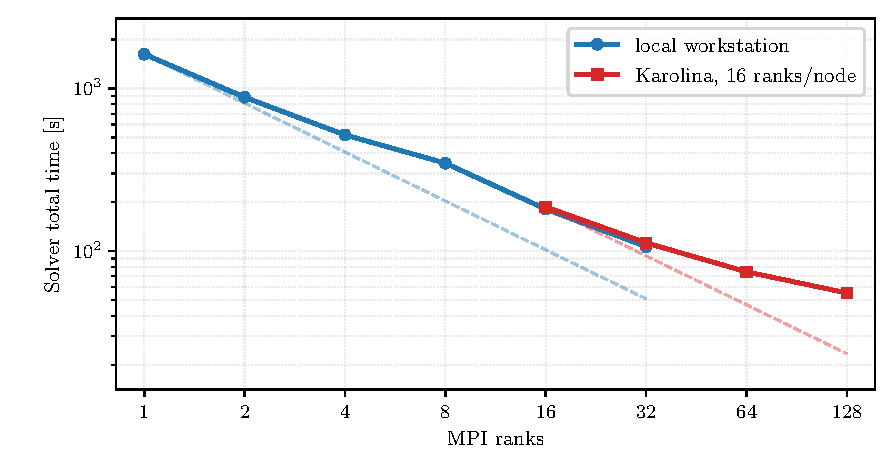
\includegraphics[width=\PaperFigureMedium]{plasticity3d_local_vs_karolina_scaling.pdf}
  \caption{Local and Karolina fixed-work scaling for the glued-bottom
  Plasticity3D $P_4(L_2)$ case at $\lambda_{\mathrm{sr}}=\num{1.55}$. Dashed
  references are ideal $1/r$ lines anchored separately to the first point of
  each platform.}
  \label{fig:plasticity3d-local-karolina-scaling}
\end{figure}

\begin{table}[H]
  \centering
  \begin{tabular*}{\textwidth}{@{}l@{\extracolsep{\fill}} c c c c c c c@{}}
\toprule
Platform & Ranks & Nodes & Solver total [s] & Solve [s] & Krylov iters & Energy & $\|g\|$ \\
\midrule
local workstation & 1 & -- & \num{1626} & \num{1370} & 29 & \num{-3013147} & \num{488.443} \\
local workstation & 2 & -- & \num{884} & \num{733} & 29 & \num{-3013147} & \num{488.443} \\
local workstation & 4 & -- & \num{518} & \num{420} & 29 & \num{-3013147} & \num{488.443} \\
local workstation & 8 & -- & \num{347} & \num{298} & 29 & \num{-3013147} & \num{488.443} \\
local workstation & 16 & -- & \num{181} & \num{155} & 29 & \num{-3013147} & \num{488.443} \\
local workstation & 32 & -- & \num{106} & \num{90.9} & 29 & \num{-3013147} & \num{488.443} \\
Karolina & 16 & 1 & \num{187} & \num{147} & 29 & \num{-3013147} & \num{488.443} \\
Karolina & 32 & 2 & \num{112} & \num{88.8} & 29 & \num{-3013147} & \num{488.443} \\
Karolina & 64 & 4 & \num{74.5} & \num{60} & 29 & \num{-3013147} & \num{488.443} \\
Karolina & 128 & 8 & \num{55.2} & \num{45.2} & 29 & \num{-3013147} & \num{488.443} \\
\bottomrule
\end{tabular*}

  \caption{Timings for the capped five-Newton-iteration Plasticity3D
  diagnostic in \cref{fig:plasticity3d-local-karolina-scaling}. Local rows are
  single-workstation MPI runs; Karolina rows use 16 ranks per CPU node.}
  \label{tab:plasticity3d-local-karolina-scaling}
\end{table}

\subsection{Topology Optimization}
\label{sec:num-topology}

The reduced design problem, mechanics subproblem, and objective history are
defined in
\Cref{sec:bench-topology,eq:topology-mechanics,eq:topology-reduced-objective}.
The numerical question here is distributed outer-loop stability: the mechanics
solve and the design update must remain synchronized under continuation in $p$
and move-regularized updates. Because the outer-loop work can vary with the
continuation schedule, the timing evidence here should be read as end-to-end
workflow scaling rather than fixed-work strong scaling.

\begin{figure}[H]
  \centering
  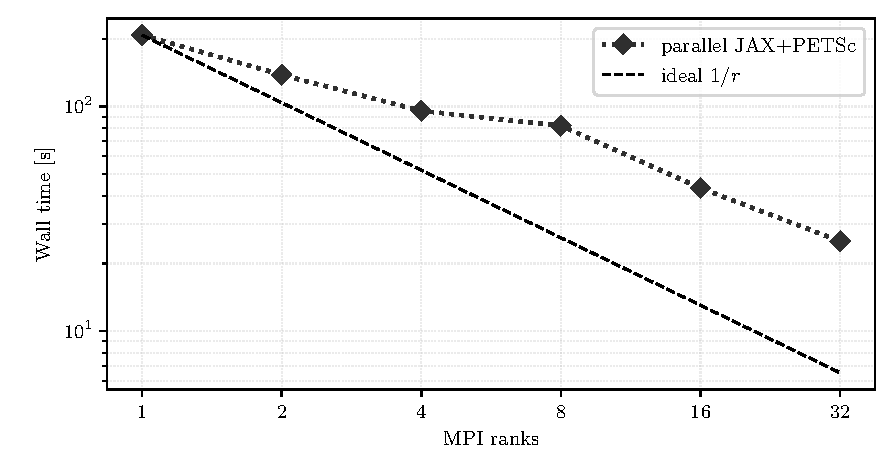
\includegraphics[width=\PaperFigureMedium]{topology_scaling.pdf}
  \caption{Topology end-to-end parallel timing trend for the maintained
  fine-grid run. The plotted wall times correspond to the coupled reduced-design
  workflow defined by \cref{eq:topology-reduced-objective}.}
  \label{fig:topology-results}
\end{figure}

\begin{table}[H]
  \centering
  \begin{tabular*}{\textwidth}{@{}c@{\extracolsep{\fill}} c c c c c c@{}}
\toprule
Ranks & Wall time [s] & Solve time [s] & Outer iters & $p$ & Compliance & Volume fraction \\
\midrule
1 & \num{208} & \num{200} & 65 & \num{4.2} & \num{9.1559} & \num{0.3884} \\
2 & \num{138} & \num{134} & 72 & \num{5.6} & \num{8.9473} & \num{0.3932} \\
4 & \num{95.7} & \num{92.8} & 69 & \num{4.6} & \num{9.1684} & \num{0.385} \\
8 & \num{82.1} & \num{80.1} & 67 & \num{7} & \num{9.2178} & \num{0.3932} \\
16 & \num{43.3} & \num{41.9} & 66 & \num{5.8} & \num{9.6859} & \num{0.3798} \\
32 & \num{25.1} & \num{23.7} & 66 & \num{6.6} & \num{9.9074} & \num{0.3749} \\
\bottomrule
\end{tabular*}

  \caption{Parallel topology summary for the maintained fine-grid study,
  reported for the reduced objective in \cref{eq:topology-reduced-objective}.}
  \label{tab:topology-summary}
\end{table}

The topology benchmark completes the paper's computational picture. Here the
mainline \jaxpetsc{} path is less about exact Hessians than about stable
distributed design-mechanics coupling, while \purejax{} remains the compact
serial reference path discussed earlier in \Cref{tab:reference-availability}.


\section{Additional Solver Evidence}
\label{sec:solver-evidence}

This section collects supporting solver evidence that is methodologically useful
but too implementation-specific for the main benchmark narratives.

\subsection{Plasticity3D Source-Assembly and Fixed-Operator PMG Comparisons}

The primary Plasticity3D numerical story in \Cref{sec:num-plasticity3d} is the
maintained local path. The tables below add two engineering comparisons on the
same discrete problem from \cref{eq:plasticity3d-discrete}: a matched
source-assembly comparator and a fixed source-operator PMG variant.

\begin{table}[H]
  \centering
  \begin{tabular*}{\textwidth}{@{}c@{\extracolsep{\fill}} c c c c c@{}}
\toprule
Ranks & Constitutive wall [s] & Source wall [s] & Constitutive solve [s] & Source solve [s] & Ratio \\
\midrule
4 & \num{1717} & \num{951} & \num{1634} & \num{890} & \num{1.805} \\
8 & \num{1164} & \num{697} & \num{1107} & \num{656} & \num{1.671} \\
16 & \num{608} & \num{374} & \num{575} & \num{350} & \num{1.628} \\
32 & \num{300} & \num{277} & \num{284} & \num{260} & \num{1.085} \\
\bottomrule
\end{tabular*}

  \caption{Matched local-vs-source comparison for the same local PMG solver
  stack. At each listed rank the local and source rows converge in the same
  number of nonlinear and linear iterations, so this is a timing-only
  comparison on \cref{eq:plasticity3d-discrete}.}
  \label{tab:plasticity3d-local-vs-source}
\end{table}

\begin{table}[H]
  \centering
  \begin{tabular*}{\textwidth}{@{}c@{\extracolsep{\fill}} l c c c c c@{}}
\toprule
Ranks & Route & Wall time [s] & Newton iters & Krylov iters & Final gradient norm & Status \\
\midrule
4 & constitutive-AD PMG solver & \num{2116} & 24 & 204 & $\num{6.53}\times 10^{-3}$ & completed \\
4 & source-assembly PMG variant & \num{988} & 21 & 210 & $\num{2.49}\times 10^{-3}$ & completed \\
8 & constitutive-AD PMG solver & \num{1874} & 33 & 238 & $\num{2.53}\times 10^{-3}$ & completed \\
8 & source-assembly PMG variant & \num{898} & 27 & 246 & $\num{9.53}\times 10^{-3}$ & completed \\
16 & constitutive-AD PMG solver & \num{1304} & 50 & 196 & $\num{2.21}\times 10^{2}$ & failed \\
16 & source-assembly PMG variant & \num{601} & 50 & 177 & $\num{7.35}\times 10^{2}$ & failed \\
32 & constitutive-AD PMG solver & \num{348} & 29 & 250 & $\num{2.24}\times 10^{-3}$ & completed \\
32 & source-assembly PMG variant & \num{398} & 50 & 193 & $\num{8.25}\times 10^{1}$ & failed \\
\bottomrule
\end{tabular*}

  \caption{Fixed source-operator PMG alternative on the same Plasticity3D
  problem. The status column distinguishes completed rows from rank counts
  that hit the Newton cap before reaching the promoted gradient target.}
  \label{tab:plasticity3d-fixed-source-pmg}
\end{table}

These tables support two narrower statements. First, source assembly has lower
reported wall time than maintained local assembly when both are embedded in the
same PMG solver stack, although the gap narrows at higher rank counts. Second,
the fixed source-operator PMG profile is not the preferred maintained default in the
present study: it may appear favorable on some rows, but it does more nonlinear
and Krylov work and converges less consistently across the reported runs.

\subsection{Source continuation evidence}

The legacy source-continuation path is not the mainline method of the paper,
but it is still useful because it isolates how much preconditioner policy
matters even when the outer continuation logic is held fixed.

\begin{table}[H]
  \centering
  \begin{tabular*}{\textwidth}{@{}l@{\extracolsep{\fill}} c c c c c@{}}
\toprule
Policy & Ranks & Runtime [s] & Init Krylov iters & Continuation Krylov iters & Final $\lambda$ \\
\midrule
fixed PMG-shell smoother & 8 & \num{489} & 58 & 733 & \num{1.568403} \\
fixed PMG-shell smoother & 32 & \num{198} & 60 & 829 & \num{1.568334} \\
\bottomrule
\end{tabular*}

  \caption{Source continuation with the fixed PMG-shell smoother policy at 8
  and 32 ranks. This is supporting solver evidence only; it is not part of the
  paper's main maintained production story.}
  \label{tab:source-cont}
\end{table}

\subsection{Code, data, and reproducibility availability}

The implementation discussed in this paper is available at
\url{https://github.com/Beremi/fenics_nonlinear_energies}. The manuscript is
generated from the repository-local paper pipeline. The table, figure,
literature-source, asset-validation, and reproducibility-note scripts live in
\path{paper/scripts}. The generated manuscript assets live in
\path{paper/tables/generated} and \path{paper/figures/generated}. The raw
benchmark summaries used by those scripts are kept under
\path{artifacts/raw_results}. The paper build validates that the generated
assets are present before compiling the PDF. A citable source or artifact
archive DOI should be supplied in the final submission metadata if required by
the target journal; this journal-neutral draft does not assert one.


\section{Discussion}
\label{sec:discussion}

The results support four main conclusions.

\paragraph{Constitutive AD is the preferred derivative route on the flagship
Plasticity3D case.}
\Cref{fig:plasticity3d-derivative-ablation,tab:plasticity3d-derivative-ablation}
show a clean cost-quality picture on the locked
$P_4(L_1)$, $\lambda_{\mathrm{sr}}=1.5$, 8-rank case. All three routes
reach essentially the same terminal state with the same nonlinear and Krylov
counts, so the comparison is about cost rather than about different converged
solutions. On that evidence, constitutive AD is the preferred maintained route:
it preserves the scalar-energy implementation contract while reducing wall time
substantially relative to full element AD and colored SFD.

\paragraph{Validation has to be separated by claim level.}
The Plasticity3D validation ladder in
\Cref{fig:plasticity3d-validation,tab:plasticity3d-validation} changes how the
paper should phrase its mechanics claims. Same-case source-faithfulness to the
source-style surrogate implementation is strong, and that is an important
result for software credibility. The fixed-lambda source-operator comparison
also satisfies the configured endpoint field-agreement thresholds once the
source boundary condition is matched to the maintained glued-bottom mask. The
right interpretation is therefore stronger but still scoped: the maintained
implementation faithfully reproduces the intended endpoint-surrogate workflow,
yet the present evidence does not justify describing that surrogate as a
path-consistent incremental elastoplastic history solve or as a verified
numeric reproduction of the Sysala source-family papers.

\paragraph{Matched external baselines are useful when the contract is narrow.}
The hyperelastic companion comparison against JAX-FEM in
\Cref{fig:hyperelasticity-jaxfem-baseline,tab:hyperelasticity-jaxfem-baseline}
shows that a narrow, fairness-first external baseline can survive review-level
scrutiny. Here the mesh and prescribed displacement schedule are matched, and
the terminal states are post-compared with the repository energy; the resulting
energy and field differences are very small. The comparison is useful precisely
because it is narrow and hyperelastic-only. The paper should not generalize it
into a broad ranking between frameworks or into plasticity validation, but it
does strengthen the manuscript by showing that at least one recent external
implementation can be matched on a shared hyperelastic problem contract.

\paragraph{Fairness and limitations remain part of the scientific result.}
Several limitations should stay explicit. The promoted Plasticity3D strong
scaling study at $\lambda_{\mathrm{sr}}=1.0$ is historical workflow
evidence, not a direct continuation of the glued-bottom
$\lambda_{\mathrm{sr}}=1.55$ matched-comparison figures. The topology study is
reported as end-to-end workflow scaling rather than fixed-work strong scaling.
Some source/local PMG studies remain solver-engineering diagnostics rather than
fully symmetric scientific baselines. None of these caveats erase the paper's
main contribution, but they do define its proper scope: a maintained
software-and-methods workflow with explicit derivative-route choices, explicit
validation surfaces, and explicit fairness boundaries.

The broader methodological lesson is that differentiable FEM becomes most
scientifically useful when local differentiation and sparse solver engineering
are designed together. Automatic differentiation alone does not settle the
behavior of large nonlinear FEM workflows; globalization, sparse ownership,
preconditioning, and the interpretation of surrogate models matter just as
much. Within that scoped claim, \repo{} contributes a reproducible maintained
workflow rather than a universal differentiable-PDE platform or a new
constitutive theory.


\section{Conclusion}
This paper presented \repo{} as a software-and-methods workflow for nonlinear
finite-element solves and optimization with a maintained \jaxpetsc{} production
path. The central contribution is not a new constitutive theory or a universal
differentiable-PDE abstraction, but a maintained implementation pattern in
which local JAX differentiation, sparse PETSc nonlinear solves, and multiple
second-order routes are kept together across a heterogeneous benchmark suite.

The Plasticity3D evidence is intentionally narrower than a broad mechanics
claim. Same-case source-faithfulness to the source-style surrogate
implementation is strong, while the fixed-lambda source-operator comparison
does not support constitutive-equivalence language. The correct reading is
therefore that the repository provides a supported maintained surrogate
workflow for this benchmark family, with constitutive AD emerging as the
preferred cost-quality route on the locked flagship case. On Hyperelasticity,
the matched companion baseline against JAX-FEM shows that the maintained code
can agree very closely with a recent external implementation when the problem
contract is made genuinely symmetric. The promoted historical Plasticity3D
scaling campaign and the distributed topology workflow then show that the same
codebase remains operational beyond small matched comparisons.

Future work should follow the boundaries made visible by these results:
\begin{itemize}
  \item extend the validation surface for path-dependent mechanics beyond the
        present surrogate-versus-source-operator comparison, including a true
        incremental-history reference;
  \item add more fairness-first external baselines on tightly matched problem
        contracts;
  \item continue reducing linear-setup and multigrid costs in the flagship 3D
        mechanics workflows.
\end{itemize}

The next scientific step is not to overclaim this implementation, but
to turn this maintained workflow into a stronger reusable template for
additional nonlinear multiphysics and design problems with equally explicit
validation and fairness criteria.


\bibliographystyle{unsrtnat}
\bibliography{references}

\end{document}
